% Options for packages loaded elsewhere
\PassOptionsToPackage{unicode}{hyperref}
\PassOptionsToPackage{hyphens}{url}
\PassOptionsToPackage{dvipsnames,svgnames*,x11names*}{xcolor}
%
\documentclass[
  12pt,
]{article}
\usepackage{amsmath,amssymb}
\usepackage{lmodern}
\usepackage{ifxetex,ifluatex}
\ifnum 0\ifxetex 1\fi\ifluatex 1\fi=0 % if pdftex
  \usepackage[T1]{fontenc}
  \usepackage[utf8]{inputenc}
  \usepackage{textcomp} % provide euro and other symbols
\else % if luatex or xetex
  \usepackage{unicode-math}
  \defaultfontfeatures{Scale=MatchLowercase}
  \defaultfontfeatures[\rmfamily]{Ligatures=TeX,Scale=1}
\fi
% Use upquote if available, for straight quotes in verbatim environments
\IfFileExists{upquote.sty}{\usepackage{upquote}}{}
\IfFileExists{microtype.sty}{% use microtype if available
  \usepackage[]{microtype}
  \UseMicrotypeSet[protrusion]{basicmath} % disable protrusion for tt fonts
}{}
\makeatletter
\@ifundefined{KOMAClassName}{% if non-KOMA class
  \IfFileExists{parskip.sty}{%
    \usepackage{parskip}
  }{% else
    \setlength{\parindent}{0pt}
    \setlength{\parskip}{6pt plus 2pt minus 1pt}}
}{% if KOMA class
  \KOMAoptions{parskip=half}}
\makeatother
\usepackage{xcolor}
\IfFileExists{xurl.sty}{\usepackage{xurl}}{} % add URL line breaks if available
\IfFileExists{bookmark.sty}{\usepackage{bookmark}}{\usepackage{hyperref}}
\hypersetup{
  colorlinks=true,
  linkcolor=blue,
  filecolor=Maroon,
  citecolor=Blue,
  urlcolor=Blue,
  pdfcreator={LaTeX via pandoc}}
\urlstyle{same} % disable monospaced font for URLs
\usepackage[margin=1in]{geometry}
\usepackage{graphicx}
\makeatletter
\def\maxwidth{\ifdim\Gin@nat@width>\linewidth\linewidth\else\Gin@nat@width\fi}
\def\maxheight{\ifdim\Gin@nat@height>\textheight\textheight\else\Gin@nat@height\fi}
\makeatother
% Scale images if necessary, so that they will not overflow the page
% margins by default, and it is still possible to overwrite the defaults
% using explicit options in \includegraphics[width, height, ...]{}
\setkeys{Gin}{width=\maxwidth,height=\maxheight,keepaspectratio}
% Set default figure placement to htbp
\makeatletter
\def\fps@figure{htbp}
\makeatother
\setlength{\emergencystretch}{3em} % prevent overfull lines
\providecommand{\tightlist}{%
  \setlength{\itemsep}{0pt}\setlength{\parskip}{0pt}}
\setcounter{secnumdepth}{5}
\usepackage[italian]{babel} \usepackage{setspace}\doublespacing \usepackage{float} \usepackage{booktabs} \usepackage{longtable} \usepackage{fontspec} \usepackage{caption} \setmainfont{Times New Roman} \usepackage{booktabs} \usepackage{multirow}
\ifluatex
  \usepackage{selnolig}  % disable illegal ligatures
\fi

\author{}
\date{\vspace{-2.5em}}

\begin{document}

\newcommand*\NewPage{\newpage\null\thispagestyle{empty}\newpage\thispagestyle{empty}}

\newpage

\thispagestyle{empty}

\begin{figure}[htbp]
      \begin{center}
        
\includegraphics[width=10cm]{figure/Logo-IZSLER.png}
      \end{center}
    \end{figure}

\begin{center}
    
  \LARGE
   \textcolor{blue}{Relazione sulla Performance anno 2020 \\ dell'Istituto Zooprofilattico Sperimentale della Lombardia e dell'Emilia Romagna}
  
  \end{center}

\begin{figure}[htbp]
      \begin{center}
        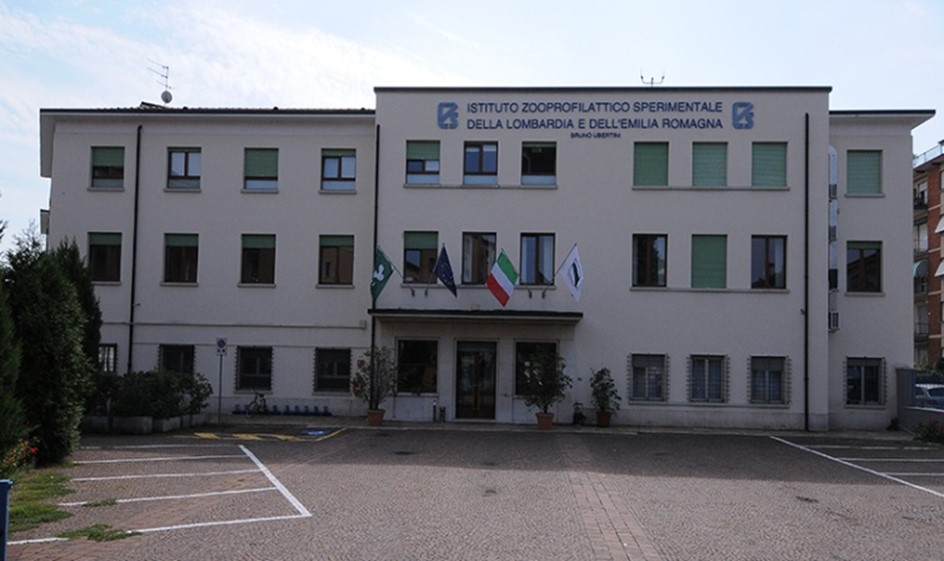
\includegraphics[width=10cm]{figure/izsler.jpg}
      \end{center}
    \end{figure}

\begin{center} 
 Adottata con Deliberazione del Consiglio di Amministrazione n. del 
 \end{center}

\begin{center}
  \small
   Istituto Zooprofilattico Sperimentale della Lombardia e dell'Emilia Romagna "Bruno Ubertini"\\
   Via A.Bianchi, 9 - 25124 Brescia- Tel. +3903022901- www.izsler.it
  \end{center}

\newpage
\tableofcontents

\newpage

\hypertarget{premessa}{%
\section*{PREMESSA}\label{premessa}}
\addcontentsline{toc}{section}{PREMESSA}

La Relazione sulla Performance, informata ai principi dell'art. 13,
comma 6, lettera b), del D Lgs n.150/2009 e all'art.10, comma 1, lettera
b) dello stesso decreto, evidenzia a consuntivo con riferimento all'anno
2020, i risultati organizzativi e individuali raggiunti rispetto agli
obiettivi programmati con rilevazione degli eventuali scostamenti. Il
documento chiude il Ciclo di Gestione della Performance avviato con
l'approvazione del ``Piano della Performance 2020-2022'' con
deliberazione del Consiglio di Amministrazione n.~2 del 24.02.2020. La
logica sottesa è quella di rendere edotti i diversi portatori di
interesse (stakeholders) sui risultati attesi ed alle modalità con cui
quei risultati sono stati raggiunti. In riferimento alle finalità sopra
descritte, si è impostata la Relazione in modo snello e comprensibile
raccogliendo le informazioni di maggior interesse ed ispirandosi ai
principi di trasparenza, immediata intelligibilità, veridicità e
verificabilità dei contenuti, partecipazione e coerenza interna ed
esterna. La presente Relazione della Performance è stata sottoposta alla
validazione del Nucleo di Valutazione delle Prestazioni e pubblicata
nella sezione «Amministrazione trasparente» del sito internet
dell'Istituto, nella sotto sezione ``Performance''.

\newpage

\hypertarget{informazioni-dinteresse-per-i-cittadini-e-gli-altri-stakeholders-esterni}{%
\section{Informazioni d'interesse per i cittadini e gli altri
stakeholders
esterni}\label{informazioni-dinteresse-per-i-cittadini-e-gli-altri-stakeholders-esterni}}

\hypertarget{gli-stakeholders-dellizsler}{%
\subsection{Gli stakeholders
dell'IZSLER}\label{gli-stakeholders-dellizsler}}

Molteplici sono i soggetti portatori di interesse o stakeholders che
hanno correlazioni di diversa natura con l'Istituto. Da quelli che
detengono un rapporto diretto, clienti, fornitori, cittadini, a tutti
gli attori le cui azioni possono direttamente o indirettamente
influenzare le scelte attuate o da porre in essere (collettività,
Pubblica Amministrazione, istituzioni pubbliche ecc.)

\begin{center}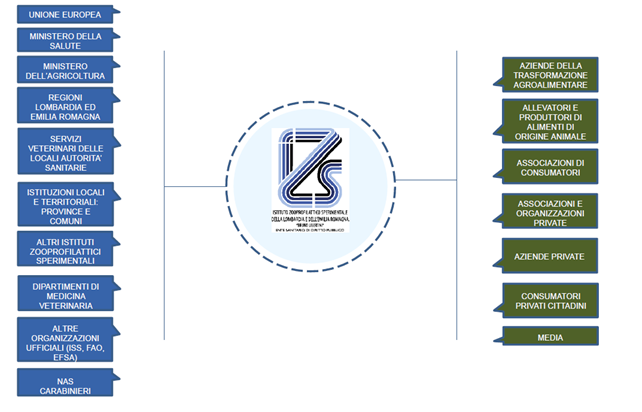
\includegraphics[width=0.9\linewidth]{figure/f1} \end{center}

\newpage

\hypertarget{analisi-del-contesto-di-riferimento}{%
\subsection{Analisi del contesto di
riferimento}\label{analisi-del-contesto-di-riferimento}}

L' analisi del contesto di riferimento ci offre la possibilità di
valutare i dati qualitativi e quantitativi che caratterizzano gli ambiti
di riferimento dell'Istituto, con l'obiettivo di fornire informazioni
rilevanti per gli stakeholders, per l'interpretazione dei risultati
raggiunti presentati nelle pagine successive.

\hypertarget{il-contesto-esterno-di-riferimento-contesto-europeo-ed-internazionale}{%
\subsubsection{Il contesto esterno di riferimento: contesto europeo ed
internazionale}\label{il-contesto-esterno-di-riferimento-contesto-europeo-ed-internazionale}}

Gli Istituti Zooprofilattici costituiscono una struttura sanitaria
integrata, unica in Europa, in grado di assicurare una rete di servizi
per verificare la salubrità degli alimenti e dell'ambiente, per la
salvaguardia della salute dell'uomo. La funzione di raccordo e
coordinamento delle attività degli II.ZZ.SS. è svolta dalla Direzione
Generale della sicurezza degli alimenti e della nutrizione del Ministero
della Salute che ne definisce, mediante il lavoro della Commissione
Scientifica Nazionale, le Linee guida e le tematiche principali. La rete
degli II.ZZ.SS. ben si integra e si riconosce con il valore
internazionale ``ONE HEALTH'' basato su collaborazioni intersettoriali e
formalmente riconosciuto dalla Commissione Europea, OMS, FAO, OIE,
istituti di ricerca, ONG e a molti altri. Questo approccio riconosce che
la salute delle persone, degli animali e degli ecosistemi sono
interconnesse, promuovendo una metodologia intersettoriale, e
multidisciplinare, in grado di affrontare i rischi potenziali o già
esistenti che hanno origine dall'interfaccia tra ambiente, animali e
uomo.

\hypertarget{il-contesto-nazionale}{%
\subsubsection{Il contesto nazionale}\label{il-contesto-nazionale}}

Gli Istituti Zooprofilattici Sperimentali (II.ZZ.SS.) costituiscono una
rete di eccellenza sul territorio nazionale in grado di operare di
concerto con il Ministero della Salute a stretto contatto con i Servizi
Veterinari Regionali e delle ASL. Assicurano al Servizio Sanitario
Nazionale attività diagnostica di campo e di laboratorio, di
sorveglianza epidemiologica, di ricerca e formazione, delle zoonosi, del
benessere animale e della sicurezza alimentare, nel rispetto degli
standard di qualità e di prevenzione stabiliti dall'Unione Europea. Gli
II.ZZ.SS. con le loro 10 sedi centrali dislocate sul territorio
nazionale e le 90 sezioni diagnostiche periferiche, sono sottoposti alla
vigilanza del Ministero della Salute.

\hypertarget{il-contesto-regionale-lombardia-e-emilia-romagna}{%
\subsubsection{IL contesto Regionale: Lombardia e Emilia
Romagna}\label{il-contesto-regionale-lombardia-e-emilia-romagna}}

L'IZSLER ha sede legale a Brescia e si avvale di 17 sedi territoriali
situate nelle regioni Lombardia (Brescia, Bergamo, Mantova, Cremona,
Sondrio, Binago (VA), Milano, Pavia e Lodi) ed Emilia-Romagna (Bologna,
Piacenza, Parma, Reggio nell'Emilia, Modena, Forlì, Ravenna e Ferrara),
che curano e gestiscono i contatti con le realtà territoriali,
interessando un'area di circa 46.000 kmq in cui risiedono oltre 14
milioni di abitanti. I dati di seguito riportati, aggiornati al
31/12/2019 (ISTAT), forniscono un quadro delle dimensioni delle regioni
di competenza dell'IZSLER.

\begin{table}[H]
\begin{tabular}{|c|c|c|c|c|c|}
\hline
\textbf{Regione} & \textbf{Popolazione} & \textbf{Superficie (km²)} & \textbf{Densità (ab/km²)} & \textbf{Comuni} & \textbf{Province} \\ \hline
Lombardia        & 10103969             & 23863,65                  & 423,4                     & 1506            & 12                 \\ \hline
Emilia-Romagna   & 4467118              & 22452,78                  & 198,96                    & 328             & 9                  \\ \hline
\end{tabular}

\end{table}

La \textbf{Regione Lombardia} può considerarsi come la ``locomotiva
d'Italia'' essendo la Regione più ricca e popolosa del Paese, nonché una
delle aree più industrializzate dell'intero panorama europeo. La
situazione economica della Regione, come emerso da un recente report
della Banca d'Italia, ha risentito pesantemente degli effetti
dell'epidemia da COVID-19 che ha colpito l'intera popolazione mondiale
nel corso del 2020 e delle restrizioni delle attività disposte dai
decreti governativi per contenere la diffusione del contagio. In
particolare, secondo le stime basate sull'indicatore trimestrale
dell'economia regionale (ITER) della Banca d'Italia, in Lombardia il
prodotto interno lordo sarebbe diminuito di circa il 12\% nei primi sei
mesi del 2020. Il recupero registrato nel terzo trimestre delle
componenti del fondo dell'economia regionale non ha compensato i cali
della prima parte dell'anno e l'attività economica è rimasta su livelli
significativamente inferiori a quelli precedenti alla crisi sanitaria.
Nell'industria, la produzione manifatturiera, secondo i dati di Union
camere Lombardia, è diminuita in misura marcata nel primo semestre
dell'anno, con un calo più accentuato nel secondo trimestre, per poi
tornare leggermente a crescere nel corso del terzo trimestre, anche se
in riduzione rispetto allo stesso periodo del 2019 (-5,2\%). Nei
servizi, il fatturato delle imprese del commercio al dettaglio si è
ridotto del 7,3\% nei primi nove mesi dell'anno rispetto ai dati dello
stesso periodo del 2019. L'impatto della pandemia è stato più contenuto
nei servizi alle imprese (-8,5\% nel primo semestre dell'anno), mentre
più intenso per i trasporti (-15,1\%) e molto marcato nei settori della
ristorazione e dell'alloggio (-34,5\%)3. Il settore dell'agricoltura
lombarda risulta il meno penalizzato dagli effetti negativi della crisi
sanitaria da COVID-19, nonostante la diminuzione del valore aggiunto
dell'agricoltura (-4,9\%) nei primi 6 mesi dell'anno, dopo un 2019
positivo. Per quanto riguarda gli scambi con l'estero, nel primo
semestre del 2020 le esportazioni lombarde di beni hanno subito una
forte contrazione rispetto al medesimo periodo del 2019 (-15,9\%) e lo
stesso dicasi per le importazioni. La crisi sanitaria legata
all'epidemia da COVID-19 ha determinato nel corso del 2020 un
progressivo peggioramento delle condizioni del mercato del lavoro. Dopo
essere stati sostanzialmente invariati durante il primo trimestre
dell'anno, gli occupati sono diminuiti in maniera significativa nel
secondo trimestre (-1,3\%) rispetto allo stato periodo del 2019,
soprattutto tra i lavoratori autonomi e tra i dipendenti con contratti
diversi dal tempo indeterminato.

La \textbf{Regione Emilia-Romagna} rappresenta, nel panorama italiano,
una delle più estese dal punto di vista territoriale, nonché più
popolose ed è una delle Regioni con il più alto livello di competitività
imprenditoriale, grazie ad un sistema economico e produttivo focalizzato
sui mercati internazionali. La crisi innescata dalla pandemia da
COVID-19 ha colpito anche l'economica delle Regione Emilia, già in
recessione dal 2019, soprattutto nei primi due trimestri dell'anno, come
evidenziato dall'indicatore trimestrale dell'economia regionale (ITER)
elaborato dalla Banca d'Italia. La riduzione della produzione
industriale della Regione (-14,9\% nella prima metà del 2020 rispetto al
medesimo periodo del 20196), ha riguardato tutti i settori della
manifattura. In tale contesto solo le imprese farmaceutiche e alimentari
hanno registrato una dinamica migliore. Nel settore dei servizi si
registra un calo generalizzato delle attività. Nel terziario, la
diminuzione dei volumi di attività è stata più evidente per il commercio
dei beni non alimentari, soprattutto al dettaglio, e per i servizi di
alloggio. Tra gennaio e settembre anche le esportazioni di merci sono
diminuite significativamente (- 14,2\%), soprattutto nell'ambito della
meccanica, dei mezzi di trasporto, dell'abbigliamento e dei prodotti di
metallo. Dopo una prolungata fese espansiva in atto dal 2014, anche il
tasso di occupazione si è ridotto, soprattutto nel secondo trimetre
dell'anno (-69,1\%), interessando principalmente la componente femminile
e quella a tempo determinato. Di seguito sono riportati alcuni dati
significativi a rappresentare il patrimonio zootecnico e le aziende che
operano nel territorio di competenza dell'Istituto.

\begin{center}
\begin{table}[H]
\begin{tabular}{|l|c|c|l|l|c|c|}
\cline{1-3} \cline{5-7}
\multicolumn{3}{|c|}{\textbf{Lombardia}}                                                               &  & \multicolumn{3}{c|}{\textbf{Emilia-Romagna}}                                    \\ \cline{1-3} \cline{5-7} 
\textbf{Specie}   & \multicolumn{1}{l|}{\textbf{N.Allevamenti}} & \multicolumn{1}{l|}{\textbf{N.Capi}} &  & \multicolumn{1}{c|}{\textbf{Specie}} & \textbf{N.Allevamenti} & \textbf{N.Capi} \\ \cline{1-3} \cline{5-7} 
Bovini e bufalini & 15446                                       & 1543959                              &  & Bovini e bufalini                    & 6448                   & 572512          \\ \cline{1-3} \cline{5-7} 
Ovini e caprini   & 13130                                       & 209308                               &  & Ovini e caprini                      & 3342                   & 71487           \\ \cline{1-3} \cline{5-7} 
Suini             & 8382                                        & 4407955                              &  & Suini                                & 3779                   & 1126379         \\ \cline{1-3} \cline{5-7} 
Avicoli           & 3427                                        & 21180545                             &  & Avicoli                              & 1170                   & 41729415        \\ \cline{1-3} \cline{5-7} 
Equidi            & 20605                                       & 61085                                &  & Equidi                               & 10744                  & 35000*          \\ \cline{1-3} \cline{5-7} 
\end{tabular}
\tiny Fonte Banca Dati Nazionale dell’Anagrafe Zootecnica (BDN) per bovini, ovini, caprini e suini – BDR per avicoli ed equini al 31/12/2020  \\
*ultima stima disponibile al 2018, dato non più presente in banca dati nazionale.

\end{table}
\end{center}

Le Regioni Lombardia ed Emilia-Romagna trattano più del 50\% del latte
italiano (300 caseifici in Emilia-Romagna e 167 in Lombardia) e oltre il
30 \% delle carni italiane con 150 impianti di macellazione in
Emilia-Romagna e 1243 in Lombardia.

\hypertarget{lamministrazione}{%
\section{L'Amministrazione}\label{lamministrazione}}

\hypertarget{un-po-di-storia-che-cosa-uxe8-listituto-zooprofilattico-sperimentale-della-lombardia-ed-emilia-romagna-izsler}{%
\subsection{Un po' di storia: Che cosa è l'Istituto Zooprofilattico
Sperimentale della Lombardia ed Emilia Romagna
(IZSLER)}\label{un-po-di-storia-che-cosa-uxe8-listituto-zooprofilattico-sperimentale-della-lombardia-ed-emilia-romagna-izsler}}

\emph{Ente Sanitario di Diritto Pubblico}, nato nel 1921, \emph{svolge
attività di supporto tecnico-scientifico in materia di salute e tutela
animale, sicurezza alimentare, salute e integrità dell'ambiente
attraverso attività analitiche, attività di analisi del rischio e di
ricerca specialistica} La rete di relazioni di IZSLER si colloca
primariamente nel tessuto sociale ed economico delle Regioni Lombardia
ed Emilia-Romagna, ma si estende a livello nazionale con le attività
istituzionali connesse con il Ministero della Salute e l'opera dei
Centri di Referenza Nazionali, nonché a livello internazionale la
collaborazione costante con organizzazioni come OIE, EFSA e FAO
\emph{L'interconnessione tra salute umana e animale} oltre gli animali
da compagnia e di allevamento e si estende alla salute degli animali
selvatici, della biosfera e degli ecosistemi in essa presenti trova
nelle molteplici competenze di IZSLER nel settore sicurezza alimentare e
sanità pubblica la possibilità di contribuire, come testimoniato dalla
situazione attuale, a creare \emph{sinergie utili per affrontare le
emergenze riguardanti la salute dell'uomo e degli animali e le emergenze
ambientali sviluppando collaborazioni e punti di incontro tra salute
umana e veterinaria}, e favorendo la connessione dei diversi attori
della salute pubblica applicando l'approccio ``One Health''.

\hypertarget{izsler-oggi-organi-funzioni-e-settori-di-competenza}{%
\subsection{IZSLER oggi: organi, funzioni e settori di
competenza}\label{izsler-oggi-organi-funzioni-e-settori-di-competenza}}

L'IZSLER opera come \textbf{strumento tecnico-scientifico} dello Stato,
della regione Lombardia e della regione Emilia Romagna nell'ambito del
Servizio Sanitario nazionale, garantendo, in tal modo, al Ministero
della Salute, alle Regioni stesse alle aziende sanitarie le prestazioni
e la collaborazione tecnico scientifica necessarie all'espletamento
delle funzioni in materia di sanità pubblica veterinaria e sicurezza
alimentare. L'Istituto Zooprofilattico Sperimentale della Lombardia e
dell'Emilia Romagna (IZSLER) è un \textbf{Ente Sanitario di Diritto
Pubblico}, dotato di autonomia gestionale, amministrativa e tecnica, che
opera nell'ambito del Servizio Sanitario Nazionale come strumento
tecnico scientifico dello Stato, delle Regioni e delle Province
Autonome, garantendo ai Servizi Veterinari le prestazioni e la
collaborazione in materia di sanita animale, controllo di salubrità e
qualità degli alimenti di origine animale, igiene degli allevamenti e
corretto rapporto tra insediamenti umani, animali ed ambiente.

La mission dell'IZSLER è:

\textbf{``Operare a favore della salute pubblica e delle attività
produttive del settore agro-alimentare nel rispetto dei valori etici, al
fine dello sviluppo socio-economico del paese''}

\textbf{L'organizzazione attuale} dell'Istituto trova il suo fondamento
normativo nel D. Lgs n.106 del 28.06.2012, recante la
\emph{``Riorganizzazione degli enti vigilati dal Ministero della Salute,
ai sensi dell'art.2 della L. n.~183 del 04.11.2010''}, delineati poi
nelle leggi regionali della Lombardia n.22 del 24.07.2014 e
dell'Emilia-Romagna n.9 del 30.06.2014. Con Deliberazione della Giunta
Regionale della Regione Lombardia n.~XI/2622 del 16.12.2019 è stato
nominato il direttore generale, \textbf{Dr.~Piero Frazzi}. L'attuale
Direttore Generale, con proprio decreto n.25 del 07.02.2020 incaricava
Direttore Amministrativo il Dott. Giovanni Ziviani e con proprio decreto
n.24 del 07.02.2020 Direttore Sanitario, il Dott. Giuseppe Diegoli. A
seguito delle personali dimissioni del Dott. Diegoli il Direttore
Generale, con proprio decreto n.243 del 30.07.2020 incaricava Direttore
Sanitario, il \textbf{Dott. Giuseppe Merialdi}.

Gli organi dell'Istituto sono:

\begin{itemize}
\item
  DIRETTORE GENERALE: Dr.~Piero Frazzi
\item
  CONSIGLIO DI AMMINISTRAZIONE: Dott. Paolo Cozzolino -- Presidente,
  Dott. Mario Chiari - Vicepresidente, Dott. Marco Delledonne - Membro,
  Dott.ssa Flavia Piccinelli -- Membro, Dott. Maurilio Giorgi - Membro.
\item
  COLLEGIO DEI REVISORI DEI CONTI: Dott. Alberto Parzani -- Presidente,
  Dott. Marco Domenicali - Componente, Dott. Lino Pietrobono -
  Componente.
\end{itemize}

Il Nucleo di Valutazione delle Prestazioni (NVP), composto da: D.ssa
Simonetta Fedeli -- Presidente Dott. Sergio Valentini -- Componente
D.ssa Giuseppina Cruso - Componente, con funzioni analoghe a quelle
degli organismo indipendente di valutazione (OIV) è un soggetto nominato
in ogni Amministrazione Pubblica e svolge in modo indipendente alcune
importanti funzioni nel processo di misurazione e valutazione della
performance, tra cui la validazione del presente documento ai sensi
dell'art. 10 lettera b) del D. Lgs 150/2009 e s.m.i..

\newpage

In particolare, all'IZSLER sono affidate le seguenti \textbf{funzioni
istituzionali}:

\begin{itemize}
\tightlist
\item
  erogazione del servizio diagnostico delle malattie degli animali e
  delle zoonosi;
\item
  supporto tecnico-scientifico ed operativo all'azione di
  farmaco-vigilanza veterinaria;
\item
  sorveglianza epidemiologica nell'ambito della sanità animale, igiene
  delle produzioni zootecniche, igiene degli alimenti, anche mediante
  l'attivazione di centri epidemiologici;
\item
  attuazione di iniziative statali o regionali, anche in collaborazione
  con le università, per la formazione, l'aggiornamento e la
  specializzazione di veterinari e di altri operatori;
\item
  cooperazione tecnico-scientifica con istituti del settore veterinario
  anche esteri, previe intese con il Ministero della Salute;
\item
  esecuzione degli accertamenti analitici necessari alle azioni di
  polizia veterinaria e all'attuazione dei piani di profilassi,
  risanamento ed eradicazione;
\item
  esecuzione degli esami necessari all'attività di controllo sugli
  alimenti di origine animale, nonché degli esami necessari all'attività
  di controllo sull'alimentazione animale;
\item
  ricerca sperimentale sulla eziologia, patogenesi e profilassi delle
  malattie infettive diffusive degli animali;
\item
  ricerca in materia di igiene degli allevamenti e delle produzioni
  zootecniche;
\item
  supporto tecnico-scientifico ed operativo per le azioni di difesa
  sanitaria e di miglioramento delle produzioni animali;
\item
  ricerca di base e finalizzata per lo sviluppo delle conoscenze in
  materia di sicurezza alimentare e sanità veterinaria, secondo
  programmi e mediante convenzioni con università e istituti di ricerca
  italiani e stranieri, nonché su richiesta dello Stato, delle Regioni
  ed altri enti pubblici;
\item
  studio e sperimentazione di tecnologie e metodiche necessarie al
  controllo sulla salubrità degli alimenti e dell'alimentazione animale;
\item
  formazione di personale specializzato nel campo della zooprofilassi e
  salubrità degli alimenti anche presso istituti e laboratori di Paesi
  esteri;
\item
  elaborazione ed applicazione di metodi alternativi all'impiego di
  modelli animali nella sperimentazione scientifica;
\item
  consulenza ed assistenza agli allevatori per la bonifica zoosanitaria,
  per lo sviluppo e il miglioramento igienico delle produzioni animali;
\item
  produzione, commercializzazione e distribuzione di medicinali e
  prodotti necessari per la lotta alle malattie degli animali e per
  l'espletamento delle funzioni di sanità pubblica veterinaria.
\end{itemize}

I settori di competenza istituzionale dell'IZSLER sono:

\begin{itemize}
\item
  \textbf{Sanità Animale}: l'IZSLER garantisce in questo settore un
  servizio diagnostico attivo negli ambiti di maggior interesse
  zootecnico (bovino, suino, ovicaprino, avicolo, cunicolo, ittico,
  apistico e della selvaggina allevata) e nelle specie di affezione
  (cani, gatti, rettili, animali selvatici, uccelli esotici, etc.). Le
  prestazioni non si limitano alle sole analisi di laboratorio ma
  comprendono anche interventi in allevamento.
\item
  \textbf{Sicurezza Alimentare}: come previsto dalle programmazioni
  sanitarie regionali e dalla politica dell'Unione Europea, l'IZSLER
  svolge funzioni di supporto nell'ambito dei piani nazionali e 15 Cfr
  ``Piano delle Performance 2020-2022'' adottato con Delibera del
  Consiglio di Amministrazione n.2/2020. 25 regionali di controllo sugli
  alimenti nella filiera produttiva e di commercio. Tale attività è
  assicurata anche a supporto delle azioni dei Nuclei Antisofisticazioni
  e Sanità (NAS) dell'Arma dei Carabinieri e degli organi periferici del
  Ministero della Salute.
\item
  \textbf{Benessere Animale} : l'accertamento dei livelli del benessere
  animale è funzionale all'attività di certificazione delle filiere
  alimentari, in linea con le attuali direttive dell'Unione Europea
  sulla qualità delle produzioni zootecniche (intesa come qualità totale
  del processo produttivo) e sulla valorizzazione delle produzioni
  locali tipiche. I parametri che caratterizzano lo stato di benessere
  sono la sintesi di un approccio combinato, multidisciplinare, basato
  su competenze di clinica, etologia, immunologia, immunobiochimica e
  sull'applicazione di tipologie analitiche di biochimica clinica.
\item
  \textbf{Formazione}: si configura come una delle mission più
  importanti e comporta la formazione di personale specializzato nel
  campo della zooprofilassi e salubrità degli alimenti anche presso
  istituti e laboratori di paesi esteri. L'IZSLER pianifica
  strategicamente le attività in tale settore, al fine di soddisfare il
  fabbisogno formativo in coerenza con le performance aziendali,
  progettando interventi formativi ad hoc e corsi accreditati ECM.
  Inoltre, mediante convenzioni, vengono accolti in Istituto, ogni anno,
  tirocinanti, frequentatori volontari e ricercatori, ed è fornita loro
  l'opportunità di svolgere attività di supporto tecnico-scientifico
  nell'ambito del corso di studi o del percorso post-laurea, delle
  scuole di specializzazione e dei dottorati di ricerca.
\item
  \textbf{Ricerca}: tra i compiti istituzionali principali dell'IZSLER
  figura l'attività di Ricerca.
\end{itemize}

I principali programmi di ricerca finanziati dal Ministero della Salute,
ai quali partecipa l'IZSLER sono:

\begin{itemize}
\item
  \textbf{la Ricerca Corrente} (è l'attività di ricerca scientifica
  diretta a sviluppare nel tempo le conoscenze fondamentali in settori
  specifici della biomedicina e della sanità pubblica);
\item
  \textbf{la Ricerca Finalizzata} (è uno dei principali strumenti per il
  conseguimento degli obiettivi delle politiche del Servizio Sanitario
  Nazionale).
\end{itemize}

L'Istituto partecipa, inoltre, a progetti di ricerca europei e ad altri
programmi di ricerca diversi da quelli finanziati dal Ministero della
Salute, a progetti finanziati dalle Regioni Lombardia ed Emilia Romagna.
L'Istituto, nell'ambito dei propri compiti istituzionali, può sviluppare
anche attività di ricerca autofinanziate (progetti autofinanziati).

Nella seguente tabella sono riportati i dati suddivisi per tipologia dei
progetti di ricerca relativamente al 2020.

\begin{center}
\begin{table}[H]
\begin{tabular}{ccccc}
\multicolumn{5}{c}{\textbf{Progetti di Ricerca Anno 2020}}                                                                                     \\ \hline
\multicolumn{1}{|c|}{\textbf{Tipologia}} &
  \multicolumn{1}{c|}{\textbf{In corso}} &
  \multicolumn{1}{c|}{\textbf{Conclusi}} &
  \multicolumn{1}{c|}{\textbf{Nuovi}} &
  \multicolumn{1}{c|}{\textbf{Totale}} \\ \hline
\multicolumn{1}{|c|}{Corrente}       & \multicolumn{1}{c|}{88}  & \multicolumn{1}{c|}{12} & \multicolumn{1}{c|}{14} & \multicolumn{1}{c|}{114} \\ \hline
\multicolumn{1}{|c|}{Autofinanziato} & \multicolumn{1}{c|}{8}   & \multicolumn{1}{c|}{3}  & \multicolumn{1}{c|}{8}  & \multicolumn{1}{c|}{19}  \\ \hline
\multicolumn{1}{|c|}{Altro tipo}     & \multicolumn{1}{c|}{3}   & \multicolumn{1}{c|}{6}  & \multicolumn{1}{c|}{4}  & \multicolumn{1}{c|}{13}  \\ \hline
\multicolumn{1}{|c|}{Istituzionale}  & \multicolumn{1}{c|}{4}   & \multicolumn{1}{c|}{5}  & \multicolumn{1}{c|}{4}  & \multicolumn{1}{c|}{13}  \\ \hline
\multicolumn{1}{|c|}{Europeo}        & \multicolumn{1}{c|}{3}   & \multicolumn{1}{c|}{3}  & \multicolumn{1}{c|}{1}  & \multicolumn{1}{c|}{7}   \\ \hline
\multicolumn{1}{|c|}{Finalizzato}    & \multicolumn{1}{c|}{4}   & \multicolumn{1}{c|}{1}  & \multicolumn{1}{c|}{0}  & \multicolumn{1}{c|}{5}   \\ \hline
\multicolumn{1}{|c|}{Regionali}      & \multicolumn{1}{c|}{1}   & \multicolumn{1}{c|}{1}  & \multicolumn{1}{c|}{3}  & \multicolumn{1}{c|}{5}   \\ \hline
\multicolumn{1}{|c|}{CCM*}           & \multicolumn{1}{c|}{2}   & \multicolumn{1}{c|}{0}  & \multicolumn{1}{c|}{0}  & \multicolumn{1}{c|}{2}   \\ \hline
\multicolumn{1}{|c|}{Totale}         & \multicolumn{1}{c|}{113} & \multicolumn{1}{c|}{31} & \multicolumn{1}{c|}{34} & \multicolumn{1}{c|}{178} \\ \hline
\multicolumn{5}{l}{*Centro Controllo Malattie}                                                                                                
\end{tabular}
\end{table}
\end{center}

\hypertarget{lattivituxe0-analitica}{%
\subsection{L'attività analitica}\label{lattivituxe0-analitica}}

L'Istituto si occupa di diagnosi delle malattie degli animali e delle
zoonosi, di controllo sugli alimenti e mangimi riguardo la presenza di
contaminanti chimici, biologici e fisici degli alimenti, di sorveglianza
epidemiologica, di ricerca e sperimentazione su tutte le materie
indicate, di formazione permanente, di supporto tecnico scientifico .La
nostra organizzazione attuale prevede l'esecuzione di diversi tipi di
attività nei laboratori della sede centrale e nelle sedi territoriali
dislocate nella regione Lombardia ed Emilia Romagna. Per ogni ulteriore
approfondimento si rimanda agli ambiti di attività presenti sulla home
page dell'Istituto.

\hypertarget{centri-di-referenza-nazionali-internazionali-e-i-laboratori-di-riferimento}{%
\subsection{Centri di referenza nazionali, internazionali e i laboratori
di
riferimento}\label{centri-di-referenza-nazionali-internazionali-e-i-laboratori-di-riferimento}}

I Centri di referenza sono strutture di eccellenza che rappresentano uno
strumento operativo di elevata e provata competenza nei settori della
sanità animale, dell'igiene degli alimenti e dell'igiene zootecnica. In
IZSLER sono attivi \textbf{9} Centri di Referenza Nazionali, \textbf{8}
Centri di referenza o di Collaborazione Internazionale, \textbf{4}
Centri di Riferimento Regionali e un Laboratorio Nazionale di
Riferimento.

Al seguente
\href{https://www.izsler.it/chi-siamo/per-chi-e-con-chi-lavoriamo/centri-di-referenza/}{link}
si accede alla pagina istituzionale dei Centri di Referenza dell'IZSLER
per maggiori dettagli.

Nell'arco del 2020 si sootolineano le seguenti attività di rilievo che
ha visto il coinvolgimento del CR\ldots..

\hypertarget{le-risorse-umane}{%
\subsection{Le risorse umane}\label{le-risorse-umane}}

Le risorse umane rappresentano il capitale primario per dell'Istituto
che investe nell'acquisizione di diverse professionalità anche ad alto
livello di specializzazione. Alla data del 31.12.2020 l'IZSLER ha nel su
organico n.~704 unità così suddivise: - 584 dipendenti assunti a tempo
indeterminato; - 57 dipendenti assunti a tempo determinato; - 50 borse
di studio; - 13 personale addetto alla ricerca;

\textbf{mettere tabelle o grafico vedi pag 15 docu word}

\hypertarget{pari-opportunituxe0-e-bilancio-di-genere}{%
\subsection{Pari opportunità e bilancio di
genere}\label{pari-opportunituxe0-e-bilancio-di-genere}}

Già da tempo l'Istituto ha promosso politiche ed interventi atti alla
promozione delle pari opportunità. Con deliberazione del Direttore
Generale n.~408 del 12.7.2011, l'ente si è dotato di un organismo che
vigilasse sul rispetto della Legge n.125 del 10.04.1991 e ss.ii.mm.,
costituendo il ``\textbf{Comitato Unico di Garanzia per le Pari
Opportunità, la Valorizzazione del Benessere di chi lavora e contro le
Discriminazioni}''. Tale organismo persegue i seguenti obiettivi:

\begin{itemize}
\tightlist
\item
  assicurare, nell'ambito del lavoro pubblico, parità e pari opportunità
  di genere;
\item
  garantire l'assenza di qualunque forma di violenza morale o
  psicologica o di discriminazione;
\item
  favorire l'ottimizzazione della produttività del lavoro pubblico,
  migliorando l'efficienza delle prestazioni lavorative;
\item
  razionalizzare e rendere efficiente ed efficace l'organizzazione della
  Pubblica Amministrazione anche in materia di pari opportunità.
  L'Organismo è stato rinnovato con Decreto del Direttore Generale
  n.~272 del 13/12/2017. In Istituto lavorano 458 donne e 245 uomini,
  così suddivisi:
\end{itemize}

\begin{center}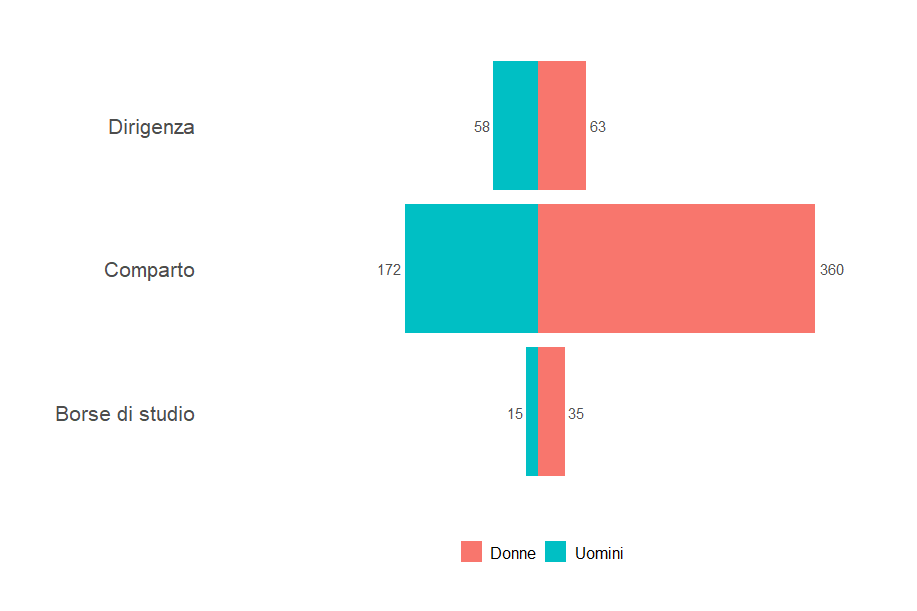
\includegraphics[width=0.9\linewidth]{figure/genere} \end{center}

\hypertarget{le-risorse-finanziarie-raggiungimento-annuale-equilibrio-di-bilancio}{%
\subsection{Le risorse finanziarie: raggiungimento annuale equilibrio di
bilancio}\label{le-risorse-finanziarie-raggiungimento-annuale-equilibrio-di-bilancio}}

Si riporta di seguito la sintesi del bilancio consuntivo anno 2019 con
le informazioni più rilevanti di carattere economico-finanziario, la
proposta di Bilancio consuntivo anno 2020 è in fase di fine istruttoria.
Nel bilancio si evidenzia un utile di esercizio pari a € 11.105.153. Per
ogni ulteriore approfondimento si rimanda alla pagina della sezione
``Amministrazione Trasparente'', sotto sezione ``Bilanci''. ll Bilancio
è stato adottato con delibera del Consiglio di Amministrazione n.~6 del
22.07.2020, il Collegio dei Revisori dei Conti ha espresso parere
favorevole con verbale n.~12 del 19.06.2020.

\begin{center}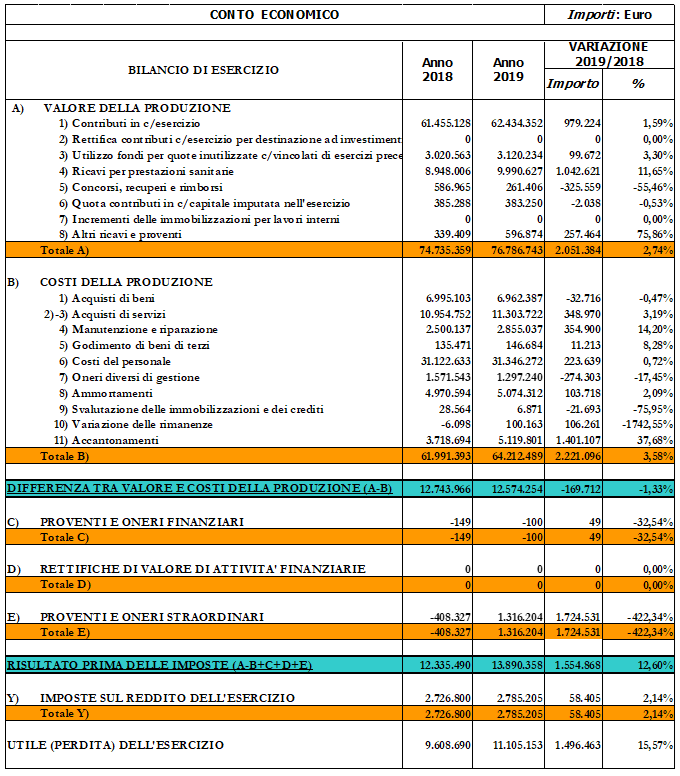
\includegraphics[width=0.9\linewidth]{figure/f6} \end{center}

\hypertarget{il-patrimonio-immobiliare}{%
\subsection{Il patrimonio immobiliare}\label{il-patrimonio-immobiliare}}

Le tabelle che seguono riportano il patrimonio immobiliare dell'Istituto
distribuito nel territorio delle due regioni di competenza.

\begin{center}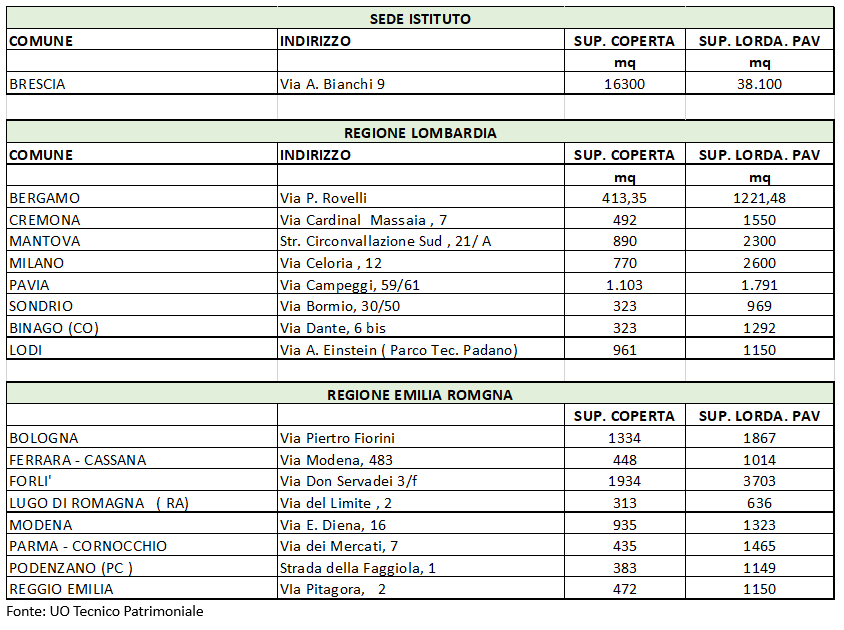
\includegraphics[width=0.9\linewidth]{figure/imm} \end{center}

\hypertarget{la-produzione-scientifica}{%
\subsection{La produzione scientifica}\label{la-produzione-scientifica}}

\hypertarget{la-formazione}{%
\subsection{La formazione}\label{la-formazione}}

L'Istituto in virtù del mandato istituzionale e della propria mission,
considera strategica l'attività della formazione e la utilizza come
strumento essenziale per favorire lo sviluppo culturale e professionale
del proprio personale. L'IZSLER è riconosciuto come provider per il
sistema di Educazione Continua in Medicina (ECM) e Centro di Referenza
Nazionale per la Sanità Pubblica Veterinaria, come tale collabora con il
Ministero della Saluta e con le Regioni di competenza per la formazione
dei veterinari e degli operatori sanitari del settore agroalimentare. Le
attività di formazione sono erogate direttamente in aule dedicate e
attrezzate e attraverso una piattaforma di Formazione a Distanza (FAD)
per corsi online, webinar e videoconferenze. La collaborazione con
Scuole superiori e Università attraverso specifiche convenzioni,
permette l'accesso ai laboratori e agli uffici di studenti delle scuole
superiori per l'alternanza scuola lavoro, degli studenti di vari
percorsi di laurea, scuole di specialità e dottorati per completare la
preparazione scolastica con la formazione sul campo. Dal 18 maggio 2012
ha conseguito la certificazione secondo la norma ``UNI EN ISO
9001:2008'', sistemi di gestione per la qualità-Requisiti'' e un
aggiornamento alla norma ``UNI EN ISO 9001:2015'' dal 18 maggio 2016.

\hypertarget{la-ricerca}{%
\subsection{La ricerca}\label{la-ricerca}}

L'attività di Ricerca figura tra i compiti istituzionali prioritari
dell'IZSLER, delineata nella legge 23 giugno 1970, n.503 (art. 3) si
attua attraverso i \textbf{\emph{programmi di ricerca finanziati dal
Ministero della Salute}}(Ricerca Corrente e Ricerca Finalizzata), ma
anche attraverso la \textbf{\emph{competizione con altri centri di
ricerca per l'accesso ai fondi europei, ai fondi dei programmi di
ricerca regionali per lo sviluppo del territorio di competenza e ai
fondi di progetti finanziati da privati}}. A sostegno delle esigenze
territoriali delle Regioni di competenza e del Ministero della salute, e
per lo sviluppo di nuovi settori IZSLER \textbf{\emph{sostiene progetti
di ricerca con finanziamento proprio}}.

IZSLER è attualmente ricercatore principale in 63 progetti dei 102 in
corso attualmente, gran parte e dei progetti sono finanziati dal
Ministero della Salute e in collaborazione con altri IIZZSS o Università

Nonostante le attività di esecuzione di migliaia di tamponi ogni giorno
ii ricercatori di IZSLER hanno collaborato con altri centri di ricerca a
livello italiano per sviluppare metodiche e approfondire le conoscenze
del virus causa di Covid 19 come ad esempio nel progetto
\textbf{\emph{Coves - Sviluppo e validazione di una metodica rapida per
la rilevazione di SARS-CoV-2 su superfici ambientali}}, ma ha
contribuito anche a ricerche di base quali quella sulle potenzialità
evolutive del coronavirus, capace di modificarsi resistendo alle difese
organiche e quella sulla possibilità di trasmissione dell'infezione da
madre a feto attraverso la placenta .

\hypertarget{il-sistema-di-gestione-integrato-di-qualituxe0}{%
\subsection{Il Sistema di Gestione Integrato di
Qualità}\label{il-sistema-di-gestione-integrato-di-qualituxe0}}

La politica dell'Istituto è orientata al miglioramento continuo della
qualità, per la creazione di un sistema di gestione dell'intera
organizzazione finalizzato al valore delle prestazioni erogate e delle
produzioni finalizzata alla soddisfazione del cliente, sia pubblico che
privato. La Direzione considera la Qualità una strategia competitiva e
parte della missione aziendale, inserendola come uno degli obiettivi da
perseguire. La qualità all'interno dell'Istituto, si traduce in un
miglioramento continuo dei servizi resi in relazione alle esigenze del
cliente e contemporaneamente alla valutazione dei costi, al fine di
soddisfare i requisiti previsti dalla legislazione nazionale e
comunitaria. A tal fine è stata definita anche una politica di
trattamento dei reclami e della soddisfazione del cliente che assicuri
che le informazioni siano comunicate alle parti direttamente coinvolte
in modo facilmente accessibile. L'Istituto sta implementando un sistema
di gestione integrato nell'ambito della qualità delle prove, delle
produzioni certificate, della sicurezza e della Biosicurezza. Gli
strumenti che l'Istituto ha individuato e di cui si avvale per il
raggiungimento di questi obiettivi sono molteplici, i principali sono:

\begin{itemize}
\tightlist
\item
  un sistema organizzato di documenti (documenti del sistema di gestione
  della Qualità) che descrivono l'applicazione degli standard di
  riferimento per la qualità all'interno dell'Ente e definiscono i
  criteri di competenza e responsabilità dei diversi ruoli deputati alla
  stesura e all'approvazione di tali documenti;
\item
  un sistema di comunicazione e diffusione per l'informazione e la
  formazione che coinvolge a cascata tutto il personale,
\item
  un sistema integrato di Audit interno che prevede una programmazione
  annuale approvata dalla Direzione Generale su proposta del RAQ e della
  Direzione Sanitaria e che contempla in un unicum le diverse tipologie
  e finalità di Audit interno.
\end{itemize}

La funzione di auditing interno integrato oltre che agire a tutela della
conformità dichiarata verso i requisiti di norma e/o legge, è per la
Direzione Generale uno strumento sistematico di conoscenza del dettato
dalle norme di riferimento per le prove e le produzioni certificate che
coadiuva l'integrazione di tali vincoli specifici con le regole degli
altri diversi sistemi che coesistono in IZSLER (Es. Biosicurezza,
Controllo di Gestione, Anticorruzione) per l'obiettivo di una maggiore
efficacia ed efficienza del Sistema di gestione inteso nell'insieme
della sue complessità e articolazioni.

Sono da segnalare nel 2020 i seguenti rilevanti cambiamenti di
organizzazione e di contesto, che hanno comportato un riesame generale
degli strumenti e dei criteri alla base della gestione per una nuova
definizione degli stessi in parte ancora da consolidare:

\begin{itemize}
\tightlist
\item
  la transizione alla nuova norma di accreditamento ISO/IEC 17025:2017
  che presenta un'importante novità con l'introduzione della gestione
  basata sul rischio;
\item
  l'applicazione della nuova organizzazione dipartimentale e le relative
  deleghe di funzioni assegnate dalla Direzione Generale ai nuovi
  Direttori di Dipartimento secondo il relativo Regolamento;
\item
  la proposta, approvata nel febbraio del corrente anno, della nuova
  organizzazione di Ente con la creazione di una nuova struttura
  complessa per il controllo di gestione per lo sviluppo dello strumento
  di budgeting dipartimentale;
\item
  l'applicazione della separazione fisica tra attività ufficiali e non
  ufficiali nell'ambito della Sicurezza Alimentare tra le diverse sedi
  territoriali/Reparti dell'Ente;
\item
  la prima applicazione, su quattro strutture sanitarie pilota,
  dell'attività di Auditing interno gestionale istituita con il Decreto
  del Consiglio di Amministrazione n.9/2020 finalizzata alla verifica in
  campo del buon governo organizzativo inclusa l'applicazione delle
  misure di contrasto alla corruzione individuate nella relativa
  mappatura del PTPCT.\\
\item
  l'integrazione della verifica delle misure di regolamentazione del
  PTPCT relative all'anonimizzazione del campione nel processo di prova
  negli Audit SAQ per la conformità ai requisiti dell'accreditamento.
\end{itemize}

Alla data del 31.12.2020 il numero totale di prove accreditate riferito
a tutte le sedi IZSLER (LAB 0148 L) è pari a 1372.

E' stata avviata ed è in corso di consolidamento una rimodulazione della
politica di accreditamento delle prove nell'ambito della Sicurezza
Alimentare, finora rivolta ove possibile alla concentrazione delle prove
accreditate per la migliore efficienza, avendo la separazione delle
attività ufficiali e di Autocontrollo, a maggiore garanzia
dell'imparzialità, comportato in alcuni casi il trasferimento delle
prove erogate prima nella stessa sede in regime di controllo ufficiale e
di autocontrollo ad altra sede presso la quale la stessa prova non
veniva eseguita. Tale maggiore impegno è compensato da un innalzamento
complessivo della qualità dei servizi erogati nelle diverse sedi
dell'Ente e di conseguenza anche dalla crescita delle competenze del
personale addetto alle attività di prova.

\hypertarget{principali-attivituxe0-e-risultati-raggiunti-dallizsler-nellanno-2020}{%
\section{Principali attività e risultati raggiunti dall'IZSLER nell'anno
2020}\label{principali-attivituxe0-e-risultati-raggiunti-dallizsler-nellanno-2020}}

\hypertarget{izsler-in-prima-linea-a-supporto-dellemergenza-da-covid-19}{%
\subsection{IZSLER: In prima linea a supporto dell'emergenza da
COVID-19}\label{izsler-in-prima-linea-a-supporto-dellemergenza-da-covid-19}}

A seguito della pandemia da covid19 che ha colpito l'Italia e il mondo,
l'Istituto è stato fin da subito in prima linea per la tutela e la
difesa della salute del cittadino, mettendo a disposizione competenze
specifiche, personale specializzato, attrezzature e ambienti idonei a
trattare patogeni ad alto rischio. Con nota prot.n. 0005086/P del
02.03.2020 il Ministero della Salute ha formalizzato il supporto
diagnostico dell'Istituto nel contrastare l'emergenza sanitaria,
individuandolo come laboratorio autorizzato per eseguire analisi, grazie
alla comprovata esperienza in campo diagnostico e alla presenza di un
Sistema di Gestione della qualità.

Già a partire da marzo 2020, l'IZSLER ha supportato il Sistema Sanitario
Nazionale nell'analisi dei tamponi nasofaringei (TNF) per la ricerca di
Sars-CoV-2 in campioni umani. Il 5 marzo è stato attivato il primo
laboratorio presso il Reparto Tecnologie Biologiche Applicate della sede
centrale di Brescia, diretto dalla dott.ssa Beatrice Boniotti, al quale
si sono aggiunti dopo pochi giorni il laboratorio presso la sede
territoriale di Pavia, diretto dalla dott.ssa Paola Prati, e
successivamente nel mese di agosto, un ulteriore laboratorio presso la
sede territoriale di Modena, diretto dalla dott.ssa Elena Carra. Ad
Ottobre è stato attivato un quarto laboratorio presso la Sede
Territoriale di Brescia, diretto dal Dr.~Alborali, dedicato all'analisi
di campioni animali e che ha supportato il primo laboratorio di Brescia
durante la seconda ondata dell'emergenza pandemica. L'IZSLER ha
codificato e validato un metodo di prova interno, MP 09/314 ``Metodo di
prova interno per la ricerca del virus Sars-CoV-2 in campioni biologici
umani mediante ``RT PCR Real Time'', sulla base dei protocolli
pubblicati sul sito del WHO e ha tenuto sotto controllo le performance
del metodo, partecipando a circuiti esterni di laboratorio promossi da
Regione Lombardia e LGC Standards. Dal 5 marzo 2020 al 31 dicembre 2020,
l'IZSLER ha analizzato n.~659.670 tamponi nasofaringei per la ricerca di
Sars-CoV-2, provenienti dalle seguenti 4 regioni:

\begin{itemize}
\tightlist
\item
  per la Lombardia sono stati analizzati n.~565.278 TNF;
\item
  per l'Emilia Romagna sono stati analizzati n.93.405;
\item
  per il Piemonte sono stati analizzati n.7;
\item
  per la Valle d'Aosta sono stati analizzati n.~980.
\end{itemize}

I tamponi provenienti da queste ultime 2 regioni sono stati analizzati
nelle primissime fasi dell'emergenza Covid, quando le Regioni, il SSN e
molti laboratori ospedalieri erano ancora in fase di organizzazione e il
numero di analisi richieste superava la capacità analitica di quelli
attivi. Mediamente sono stati analizzati 2440 tamponi al giorno con
picchi fino 5100 durante le settimane più acute della seconda ondata nei
mesi di ottobre e novembre. Per quanto riguarda le province lombarde, il
maggior numero di TNF analizzati dall'IZSLER proveniva dalla provincia
di Brescia, per un totale di 190.268 TNF, seguita dalla provincia di
Mantova con 114.546 TNF, quindi la provincia di Milano con 62.384 TNF.
Per l'Emilia Romagna invece la provincia con più TNF analizzati è stata
Bologna con 41.372, seguita dalla provincia di Parma con 21.301 e la
provincia di Piacenza con 18.515 TNF analizzati. L'IZSLER ha analizzato
tamponi provenienti da 227 diversi conferenti, la maggior parte dei
quali appartenenti a strutture ospedaliere come ASST del Garda, ASST
della Franciacorta, ASST di Mantova, ASST di Crema, Spedali Civili di
Brescia, ASST Santi Paolo e Carlo, ASST di Cremona, ASST Bergamo Ovest,
ASST di Lodi, ASST Valle Olona, ASST Ovest Milanese e ASST Lariana; tra
i conferenti anche le principali ATS locali, come ATS della Valpadana,
ATS Brescia, ATS Bergamo, ATS Pavia, ATS Brianza, ATS della Montagna;
tra i restanti conferenti numerose RSA del territorio, Fondazioni Onlus,
case di cura, strutture e cliniche private Entrando nel dettaglio per
ogni singolo laboratorio, in tutto il 2020 il laboratorio dedicato della
sede di Brescia ha refertato n.412.158 tamponi provenienti da tutte le
province della Lombardia, il laboratorio della sede territoriale di
Pavia n.~170.640 tamponi provenienti da Lombardia, Piemonte, Valle
d'Aosta ed Emilia Romagna, e la sede territoriale di Modena ha
analizzato n.~76.872 tamponi, provenienti da Lombardia ed Emilia
Romagna. La sede di Brescia ha avuto 163 diversi conferenti, tra i quali
ATS della Valpadana con 13001 tamponi analizzati, ASST del Garda con
56.215 analisi, ASST di Crema con 25713 analisi, ASST della Franciacorta
con 20.526 analisi, Spedali Civili di Brescia con 42.650 tamponi, ASSt
Santi Paolo e Carlo con 19.698 tamponi, ASST di Mantova con 81.688
analisi, ATS Bergamo con 12.275 tamponi, ATS Brescia con 2572 tamponi.
La sede di Pavia ha registrato 63 diversi conferenti, tra cui ATS Pavia
con 51.918 tamponi analizzati, Ospedale di Vigevano con 12.277 analisi,
ASST Lariana con 12.259 analisi e ASST Ovest Milanese con 17.124
analisi, AUSl di Piacenza con 18.500 analisi, ICS Maugeri-IRCCS Pavia
con 11.019 tamponi. La sede di Modena ha avuto 20 diversi conferenti,
tra cui AUSl di Bologna con 40.626 tamponi analizzati, AUSL di Parma con
11.432 analisi, AUSL Romagna con 11.874 tamponi, ATS della Valpadana con
7.748 tamponi analizzati e ASST di Mantova con 1.582 analisi.

E' da sottolineare che l'Istituto per far fronte all'emergenza sanitaria
ha dovuto prontamente riprogrammare le proprie attività, alcune delle
quali sono state momentaneamente sospese e qualche laboratorio è stato
riconvertito, per dare spazio all'esecuzione urgente di analisi dei
campioni da covid19. A tal proposito per supportare le ingenti attività
laboratoriale l'intera organizzazione dell'istituto è stata coinvolta a
vario titolo mettendo in campo le seguenti azioni:

\begin{itemize}
\tightlist
\item
  l' UO gestione personale ha assunto n.26 personale tecnico sanitario
  dedicato al campionamento;
\item
  l'UO Provveditorato ha gestito numerose gare per l'acquisizione del
  materiali necessario all'esecuzione dei campioni;
\item
  i Sistemi Informativi hanno supportato i laboratori dal punto di vista
  tecnico-informatico;
\item
  sono state revisionate tutte le procedure di sicurezza e biosicurezza
  per il personale e per garantire l'accesso in sede da parte
  dell'utenza;
\item
  sono state riviste le procedure di accettazione dei campioni, di
  acquisizione di beni e servizi specifici;
\item
  si è garantito un costante flesso informativo dei dati epidemiologici
  verso il Ministero della Salute e delle regioni;
\item
  si è provveduto ad organizzare corsi di formazione specifici per gli
  addetti ai servizi di laboratorio; Il grande lavoro di equipe/squadra
  dell'Istituto ha permesso di fronteggiare l'emergenza sanitaria con
  prontezza ed efficacia, dimostrando notevoli capacità organizzative e
  spirito di servizio.
\end{itemize}

\hypertarget{un-importante-riconoscimento-laboratorio-nazionale-di-riferimento-per-le-tossine-vegetali-naturali-negli-alimenti}{%
\subsection{Un importante riconoscimento: Laboratorio Nazionale di
Riferimento per le Tossine Vegetali Naturali negli
alimenti}\label{un-importante-riconoscimento-laboratorio-nazionale-di-riferimento-per-le-tossine-vegetali-naturali-negli-alimenti}}

Con la nota n° 0033302 DGISAN-MDS-P del 23/09/2020, in conformità
all'articolo 100 del Regolamento UE 625/2017, il Ministero della Salute
ha designato il Reparto Chimico degli Alimenti di Bologna dell'Istituto
Zooprofilattico Sperimentale della Lombardia e dell'Emilia-Romagna
(IZSLER) quale Laboratorio Nazionale di Riferimento per le tossine
vegetali naturali negli alimenti in condivisione con il Dipartimento di
Sicurezza Alimentare, Nutrizione e Sanità Pubblica Veterinaria
dell'Istituto Superiore di Sanità (ISS). Il Reparto Chimico e l'ISS
lavoreranno secondo le rispettive competenze coordinandosi e
condividendo periodicamente i programmi di lavoro, in accordo con il
comma 5 dell'articolo 100 del Regolamento UE 625/2017. L'attività degli
LNR è incentrata sullo sviluppo e sull'applicazione di metodi di analisi
per la determinazione delle tossine vegetali naturali in diverse matrici
di origine vegetale quali cereali, baby food, miele, polline, erbe
infusionali, spezie, semi di lupino e derivati, prodotti da forno a base
di semi di papavero, mandorle e armelline, olii e grassi vegetali,
prodotti alimentari a base di canapa, solanacee e integratori alimentari
a base di aloe. Le tossine vegetali su cui i laboratori operano sono:
gli alcaloidi del tropano e le calistegine, gli alcaloidi
pirrolizidinici, gli alcaloidi chinolizidinici, gli alcaloidi
dell'oppio, l'acido cianidrico, l'acido erucico, i cannabinoidi, i
glicoalcaloidi, l'idrossiantracene. Ciascun laboratorio partecipa
annualmente a prove comparative inter-laboratorio organizzate dall'EURL
``Mycotoxins \& plant toxins'' di Wageningen (Paesi Bassi) e programma
la partecipazione a circuiti di interesse organizzati da altri enti
riconosciuti con lo scopo di valutare e monitorare la competenza tecnica
del laboratorio. Inoltre entrambi i laboratori pianificano e organizzano
secondo una programmazione concordata ed in base alla specifiche
competenze prove comparative inter-laboratorio tra laboratori ufficiali
per metodi di screening e per metodi di conferma assicurando un adeguato
follow-up delle attività. I laboratori operano a stretto contatto con la
rete dei laboratori ufficiali e forniscono informazioni e supporto ai
laboratori del controllo ufficiale.

\hypertarget{progettazione-e-realizzazione}{%
\subsection{Progettazione e
realizzazione}\label{progettazione-e-realizzazione}}

Nel corso dell'anno 2020 l'attività di costruzione ha avuto un
rallentamento per la pandemia da Covid-19. I primi mesi dell'anno
l'attività si è concentrata sull'esecuzione di lavori per la
predisposizione di due laboratori per l'analisi dei tamponi Covid-19
mentre gli altri cantieri hanno visto un sostanziale fermo. Nonostante
quanto sopra precisato nell'anno 2020 si sono realizzate le seguenti
attività:

\begin{itemize}
\tightlist
\item
  la progettazione per la realizzazione della nuova accettazione unica
  presso la sede di Brescia;
\item
  la trasformazione del seminterrato dello stabulario a deposito libri;
\item
  l'inizio del cantiere per la realizzazione del nuovo laboratorio di
  Batteriologia;
\item
  la realizzazione del nuovo laboratorio entomologico di Reggio Emilia;
\item
  la realizzazione dell'ampliamento della sede di Bologna ha avuto un
  rallentamento ma si ritiene che l'attività si concluderà nell'anno
  2021;
\item
  l'inizio della progettazione definitiva ed esecutiva per la nuova sede
  territoriale di Cremona. Si sono approvate inoltre le seguenti
  progettazioni:
\item
  progetto di fattibilità tecnico- economica la ristrutturazione della
  sede territoriale di Parma;
\item
  progetto di fattibilità tecnico-economica degli ambienti lasciati
  liberi per il trasferimento della sede di Bologna per il reparto
  chimico;
\item
  completamento progettazione per la trasformazione a laboratorio
  dell'ex magazzino della sede territoriale di Reggio Emilia.
\end{itemize}

Nel 2020 si sono attivate due importanti convenzioni, una con la
Centrale Unica di Committenza (CUC) della Provincia di Brescia per
l'esperimento di alcune procedure di gara e l'altra con Infrastrutture
Lombarde (ora AREA spa) per la completa realizzazione di due importanti
interventi previsti presso la sede di Brescia.

Con la CUC della Provincia di Brescia si sono esperite le procedure di
gara come da tabella sottostante:

\begin{center}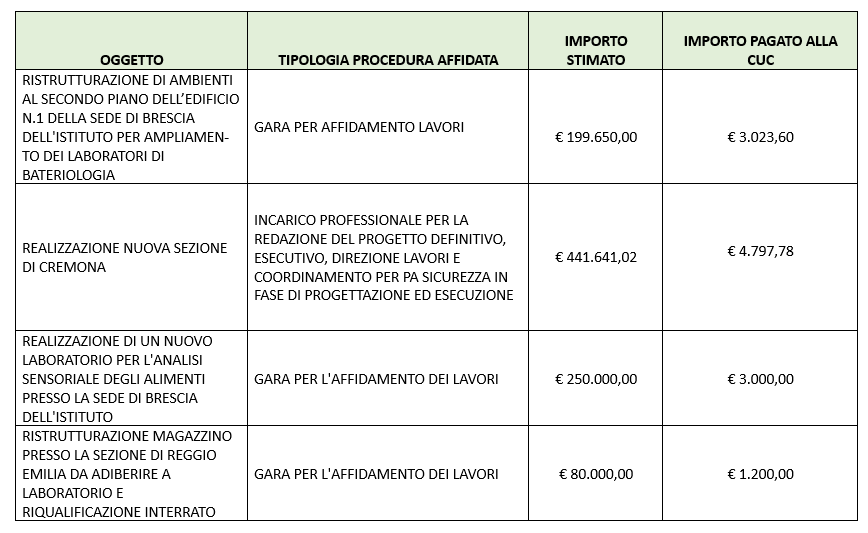
\includegraphics[width=0.9\linewidth]{figure/gare1} \end{center}

Con Infrastrutture Lombarde (ora AREA SPA) l'Istituto ha sottoscritto
una convenzione per la realizzazione di due importanti interventi
affidandone alche la funzione di Stazione Appaltante:

\begin{center}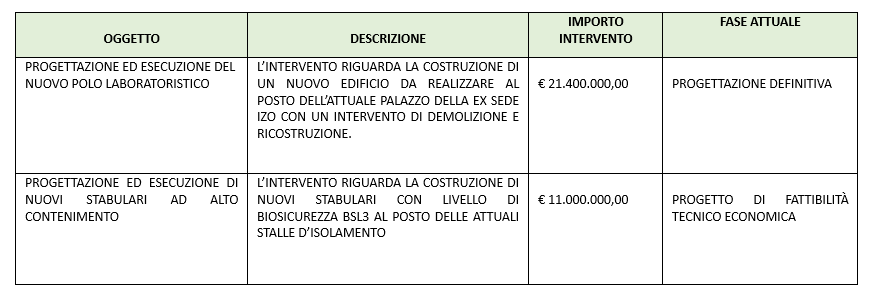
\includegraphics[width=0.9\linewidth]{figure/gare2} \end{center}

\hypertarget{aspetti-organizzativi-attuazione-dei-dipartimenti}{%
\subsection{Aspetti organizzativi: attuazione dei
dipartimenti}\label{aspetti-organizzativi-attuazione-dei-dipartimenti}}

Con Delibera del Consiglio di Amministrazione n.~17 del 15.12.2020 è
stato attuato un nuovo modello organizzativo, che ha permesso di porre
le basi per perseguire la finalità di creare un'unica identità e
integrare, capitalizzandole, le esperienze passate, mettendo a fattore
comune le buone pratiche, con il desiderio di vivere una nuova realtà
organizzativa. I criteri utilizzati per la definizione
dell'organizzazione sono:

\begin{itemize}
\tightlist
\item
  valorizzare le funzioni dell'IZSLER in tema di prevenzione, analisi
  della domanda, valutazione dei bisogni e governo dell'offerta;
\item
  delineare un'organizzazione snella ma adeguata alla complessità
  dell'IZSLER;
\item
  governare le tematiche e i processi con un'attenzione particolare
  all'articolazione territoriale;
\item
  essere garante per la salute dei cittadini, integrandosi con gli enti
  sanitari e nazionali e tutti gli attori del territorio, in sinergia
  con le istituzioni locali.
\end{itemize}

Il nuovo modello ha comportato l'attuazione dei seguenti Dipartimenti:

\begin{itemize}
\tightlist
\item
  DIPARTIMENTO SICUREZZA ALIIMENTARE
\item
  DIPARTIMENTO TUTELA SALUTE ANIMALE
\item
  DIPARTIMENTO AREA TERRITORIALE EMILIA ROMAGNA
\item
  DIPARTIMENTO AREA TERRITORIALE LOMBARDIA
\item
  DIPARTIMENTO AMMINISTRATIVO
\end{itemize}

\hypertarget{piramide-della-ricerca}{%
\subsection{Piramide della ricerca}\label{piramide-della-ricerca}}

A seguito dell'emanazione del Decreto Ministeriale 20 novembre 2019,
n.164 ``Regolamento recante la valutazione del personale della ricerca
sanitaria`` (GU serie generale n.2 del 03.01.2020) sono stati stipulati
nell'arco del 2019/2020 n.~6 contratti di Collaboratore Professionale di
ricerca sanitaria cat. D e n.~8 Ricercatore Sanitario cat. Ds, secondo
le previsioni dell'art. 1 comma 423 della Legge n.205/2017. Con decreto
del Direttore Generale n.~28 del 26.01.2021 è stato istituito il Nucleo
di Valutazione del Personale della ricerca sanitaria, costituito da:

\begin{itemize}
\tightlist
\item
  Presidente: Dott. Piero Frazzi, Direttore Generale che si avvale per
  gli aspetti di competenza del Direttore Sanitario, Dott. Giuseppe
  Merialdi;
\item
  Componente: Dott. Antonio Lavazza, Dirigente Responsabile Dipartimento
  Sanità Animale;
\item
  Componente: Dott. Guerino Lombardi, Dirigente Responsabile Struttura
  Biblioteca, Formazione e Comunicazione;
\end{itemize}

\hypertarget{ciclo-di-gestione-della-performance}{%
\section{Ciclo di gestione della
performance}\label{ciclo-di-gestione-della-performance}}

\hypertarget{una-definizione-di-performance}{%
\subsection{Una definizione di
performance}\label{una-definizione-di-performance}}

La \textbf{performance} è intesa come \emph{contributo (risultato e
modalità di raggiungimento del risultato) che le varie componenti
organizzative (individui, gruppi di individui, unità organizzative, ente
nel suo complesso) apportano attraverso la propria azione al
raggiungimento delle finalità e degli obiettivi dell'Ente ed, in ultima
istanza, alla soddisfazione dei bisogni della collettività per i quali
l'Ente è stato costituito} .Quindi la capacità di ottenere risultati per
i propri utenti e portatori d'interesse mediante il migliore utilizzo
delle risorse messe a disposizione.

\hypertarget{perchuxe9-misuriamo-e-valutiamo-la-performance-dellistituto}{%
\subsection{Perché misuriamo e valutiamo la performance
dell'Istituto}\label{perchuxe9-misuriamo-e-valutiamo-la-performance-dellistituto}}

L'attività di misurazione e valutazione della performance si colloca, al
centro della riforma del lavoro pubblico, configurata a partire dagli
anni novanta con le disposizioni normative confluite poi nel D Lgs
165/2001 e s.m.i. fino alle disposizioni della legge n.15/2009 e del D
Lgs n.150/2009 e s.m.i. L' impostazione della riforma porta al centro
dell'azione amministrativa la logica della misurazione della performance
e di risultati, in un'ottica di recupero di efficienza e di efficacia al
fine del miglioramento della qualità dell'azione della P.A. e un più
ottimale utilizzo delle risorse. Ai fini dell'attuazione dei principi di
cui all'art. 3 D Lgs 150/2009, le Pubbliche Amministrazioni, definiscono
e assegnano gli obiettivi che si intendono raggiungere, volte alla
misurazione della \textbf{performance organizzativa e individuale}.

La performance organizzativa misura la performance dell'ente
complessivamente, tramite gli obiettivi strategici, e quella delle varie
strutture, tramite gli obiettivi operativi.

\hypertarget{performance-organizzativa-di-ente-nel-suo-complesso}{%
\subsubsection{Performance organizzativa di ente nel suo
complesso}\label{performance-organizzativa-di-ente-nel-suo-complesso}}

La performance organizzativa di ente richiede per essere misurata
l'individuazione di una \textbf{batteria di obiettivi/indicatori
strategici, inseriti nel Cruscotto di Ente e approvati all'interno del
Piano Performance, che discendono da una programmazione
istituzionale/strategica}.

L'Istituto pianifica le proprie attività secondo 3 livelli di
programmazione:

\begin{enumerate}
\def\labelenumi{\alph{enumi})}
\item
  un \textbf{livello istituzionale} di ordine strategico che si
  qualifica per definire gli indirizzi di fondo pluriennali e annuali
  cui l'Istituto è tenuto, per quanto di competenza, ad attenersi;
\item
  un \textbf{livello strategico} qualificato per declinare gli indirizzi
  strategici ministeriali e regionali;
\item
  un \textbf{livello operativo} dove gli obiettivi strategici vengono
  declinati con gli strumenti di programmazione.
\end{enumerate}

Tale rappresentazione risulta per altro coerente con quanto previsto
dall'art. 27 dello Statuto: \emph{``L'Istituto, ai fini di assicurare
l'efficienza e l'efficacia dell'azione amministrativa nonché la
rispondenza dell'attività delle strutture organizzative agli indirizzi
prefissati, si dota di un proprio ciclo di gestione delle performance,
che prevede l'adozione di un piano triennale in relazione alle
performance attese, con propri indicatori e con gli strumenti di
valutazione del livello di raggiungimento delle stesse, da approvarsi
con deliberazione del consiglio di amministrazione''}.

\hypertarget{obiettivi-strategici-e-cruscotto-di-ente}{%
\subsubsection{Obiettivi strategici e cruscotto di
ente}\label{obiettivi-strategici-e-cruscotto-di-ente}}

Il Consiglio di Amministrazione con Deliberazione n.~2 del 24.02.2020 ha
dato il via al Ciclo di Gestione delle Performance, adottando il ``Piano
Performance 2020-2022'', contenente gli obiettivi strategici
dell'Istituto declinati secondo gli indirizzi Ministeriali e Regionali.
Gli obiettivi strategici, raggruppati all'interno delle diverse
``prospettive di analisi'', secondo l'approccio della Balanced
Scorecard, sono i seguenti:

\textbf{PROSPETTIVA ISTITUZIONI CITTADINI E CONSUMATORI} Prospettiva
orientata a misurare l'impatto delle azioni in termini di valore
prodotto con riferimento ai diversi portatori di interesse, valutando la
capacità dell'ente di garantirne la piena soddisfazione delle
aspettative di questi ultimi.

\begin{itemize}
\tightlist
\item
  1.IMPLEMENTAZIONE DELLE ATTIVITA' RELATIVE ALLA RICERCA NAZIONALE E
  INTERNAZIONALE
\item
  2.IMPLEMENTAZIONE DELLE ATTIVITA' ISTITUZIONALI NEL SETTORE DELLA
  SICUREZZA ALIMENTARE, SANITA' ANIMALE E IGIENE VETERINARIA
\end{itemize}

\textbf{PROSTETTIVA ECONOMICA FINANZIARIA} prospettiva orientata al
monitoraggio degli aspetti economico-finanziari in relazione alla
programmazione strategica volta, quindi, a valutare la gestione
dell'ente in ragione della sua capacità di perseguire adeguati margini.

\begin{itemize}
\item
  \begin{enumerate}
  \def\labelenumi{\arabic{enumi}.}
  \setcounter{enumi}{2}
  \tightlist
  \item
    SOSTENIBILITA' ECONOMICA E FINANZIARIA
  \end{enumerate}
\end{itemize}

\textbf{PROSPETTIVA PROCESSI INTERNI} prospettiva orientata ad
individuare il grado di efficienza ed efficacia con il quale l'Ente
gestisce e controlla i processi interni mediante l'ottimizzazione di
quelli esistenti ed alla definizione di processi attraverso i quali
perseguire gli obiettivi strategici.

\begin{itemize}
\item
  \begin{enumerate}
  \def\labelenumi{\arabic{enumi}.}
  \setcounter{enumi}{3}
  \tightlist
  \item
    REINGEGNERIZZAZIONE DEI PROCESSI
  \end{enumerate}
\end{itemize}

\textbf{PROSTETTIVA INNOVAZIONE, CRESCITA E SVILUPPO ORGANIZZATIVO}
prospettiva volta alla valorizzazione delle potenzialità interne
dell'ente per una crescita del personale in termini di competenze e
motivazione nonché al potenziamento delle infrastrutture tecniche e
tecnologiche di supporto.

\begin{itemize}
\item
  \begin{enumerate}
  \def\labelenumi{\arabic{enumi}.}
  \setcounter{enumi}{4}
  \tightlist
  \item
    AMMINISTRAZIONE TRASPARENTE ED ANTICORRUZIONE
  \end{enumerate}
\item
  \begin{enumerate}
  \def\labelenumi{\arabic{enumi}.}
  \setcounter{enumi}{5}
  \tightlist
  \item
    VALORIZZAZIONE DEL CAPITALE UMANO
  \end{enumerate}
\end{itemize}

Tale approccio ha supportato il processo di redazione del Piano della
Performance, in cui gli obiettivi dell'Istituto sono stati declinati in
una logica multidimensionale.

\begin{center}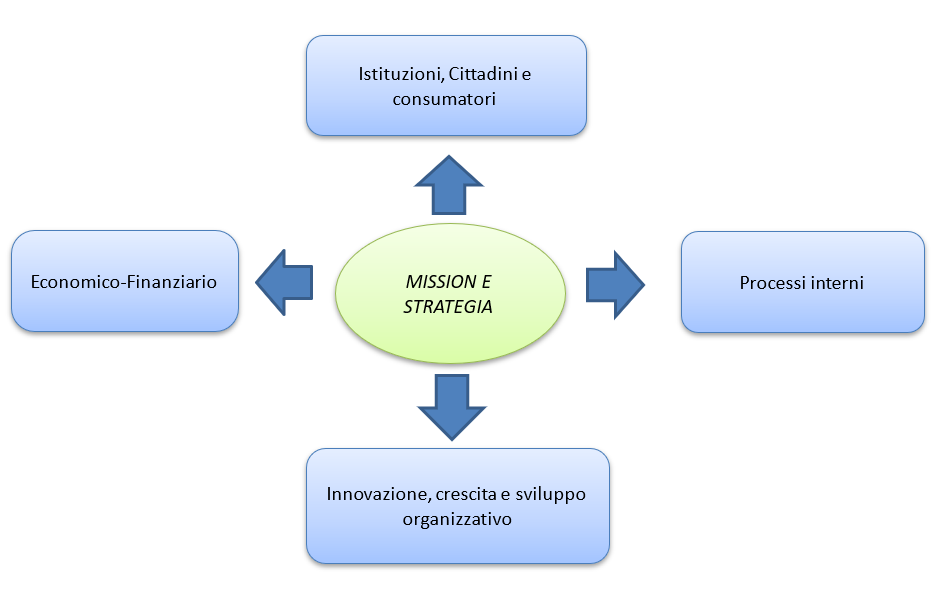
\includegraphics[width=0.9\linewidth]{figure/f2} \end{center}

Come già sopra menzionato, al fine di individuare un sistema in grado di
garantire la misurazione, valutazione e quindi, la rappresentazione in
modo integrato ed esaustivo del livello di performance atteso e
realizzato, con successiva evidenziazione di eventuali scostamenti,
l'IZSLER provvede alla costruzione del cruscotto degli indicatori
necessario per la misurazione della strategia. Infatti, una volta
definiti gli obiettivi strategici si procede all'individuazione delle
misure in grado di monitorare il loro grado di raggiungimento. Al fine
di garantire un monitoraggio continuo della performance dell`Ente, anche
ai fini dell'individuazione degli interventi correttivi in corso di
esercizio, \textbf{gli indicatori individuati devono essere in grado di
rappresentare tutte le azioni messe in atto per il raggiungimento degli
obiettivi strategici prefissati}. Nella costruzione del cruscotto,
contestualmente alla definizione degli indicatori, si procede alla
definizione dei target e degli intervalli di variazione grazie ai quali
l'Ente è in grado di rilevare lo scostamento tra i valori attesi e
quelli effettivamente realizzati ed effettuare le opportune valutazioni.
Di seguito si riporta il \textbf{Cruscotto di Ente}, che rispetto a
quello dell'anno precedente, presenta una migliore razionalizzazione
degli obiettivi strategici, dei Project e un minor numero indicatori per
ciascuno di essi, individuati comunque in modo tale da garantire una
corretta rappresentazione della performance dell'Ente, in continuità con
la mission dell'Istituto.

\hypertarget{cruscotto-dellente-anno-2020}{%
\subsection{Cruscotto dell'ente anno
2020}\label{cruscotto-dellente-anno-2020}}

Di seguito per ogni obiettivo strategico sono riportati i rispettivi
obiettivi operativi/azioni e una tabella che sintetizza gli indicatori
adottati, il target , il grado di raggiungimento e una breve descrizione
del risultato raggiunto

\hypertarget{obiettivo-strategico-1-implementazione-delle-attivituxe0-relative-alla-ricerca-nazionale-e-internazionale}{%
\subsubsection*{\texorpdfstring{Obiettivo strategico 1:
\textbf{Implementazione delle attività relative alla ricerca nazionale e
internazionale}}{Obiettivo strategico 1: Implementazione delle attività relative alla ricerca nazionale e internazionale}}\label{obiettivo-strategico-1-implementazione-delle-attivituxe0-relative-alla-ricerca-nazionale-e-internazionale}}
\addcontentsline{toc}{subsubsection}{Obiettivo strategico 1:
\textbf{Implementazione delle attività relative alla ricerca nazionale e
internazionale}}

Questo obiettivo è declinato in due azioni principali (obiettivi
operativi):

-1 Rafforzamento della competitività nell'ambito della progettualità e
della ricerca sperimentale nazionale ed internazionale

-2 Sviluppare sinergie per valorizzare le competenze dei CRN

\begin{center}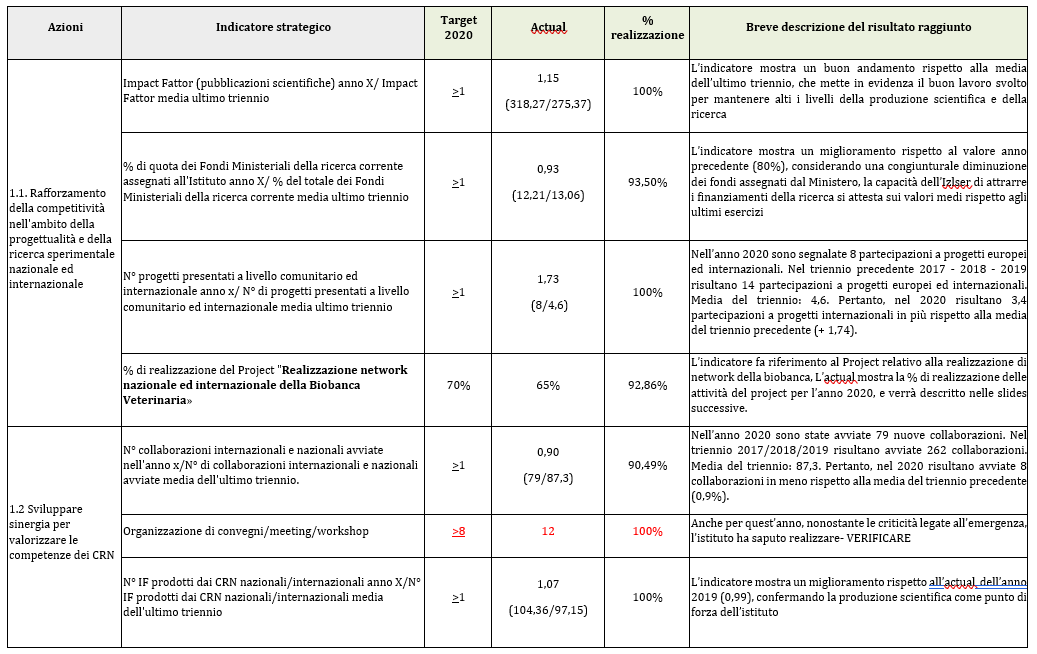
\includegraphics[width=1.1\linewidth]{figure/ob1} \end{center}

\newpage

\hypertarget{obiettivo-strategico-2-implementazione-delle-attivituxe0-istituzionali-nel-settore-della-sicurezza-alimentare-sanituxe0-animale-e-igiene-veterinaria}{%
\subsubsection*{\texorpdfstring{Obiettivo strategico 2:
\textbf{Implementazione delle attività istituzionali nel settore della
sicurezza alimentare, sanità animale e igiene
veterinaria}}{Obiettivo strategico 2: Implementazione delle attività istituzionali nel settore della sicurezza alimentare, sanità animale e igiene veterinaria}}\label{obiettivo-strategico-2-implementazione-delle-attivituxe0-istituzionali-nel-settore-della-sicurezza-alimentare-sanituxe0-animale-e-igiene-veterinaria}}
\addcontentsline{toc}{subsubsection}{Obiettivo strategico 2:
\textbf{Implementazione delle attività istituzionali nel settore della
sicurezza alimentare, sanità animale e igiene veterinaria}}

Questo obiettivo è declinato in tre azioni principali (obiettivi
operativi):

-1 Sviluppo di sistemi di analisi del dato sanitario;

-2 Potenziamento dell'attività di diagnostica, produzione, supporto
tecnico scientifico

-3 Attuazione nuove strategie per l'incremento degli interventi di
conoscenza e competenza verso l'esterno

\begin{center}\includegraphics[width=1.1\linewidth]{figure/ob2} \end{center}

\newpage

\hypertarget{obiettivo-strategico-3-sostenibilituxe0-economica-finanziaria}{%
\subsubsection*{\texorpdfstring{Obiettivo strategico 3:
\textbf{Sostenibilità economica
finanziaria}}{Obiettivo strategico 3: Sostenibilità economica finanziaria}}\label{obiettivo-strategico-3-sostenibilituxe0-economica-finanziaria}}
\addcontentsline{toc}{subsubsection}{Obiettivo strategico 3:
\textbf{Sostenibilità economica finanziaria}}

Questo obiettivo è declinato in un'unica azione (obiettivo operativo):

\begin{itemize}
\tightlist
\item
  1 Ottimizzare l'uso di risorse per aumentare l'efficienza
\end{itemize}

\begin{center}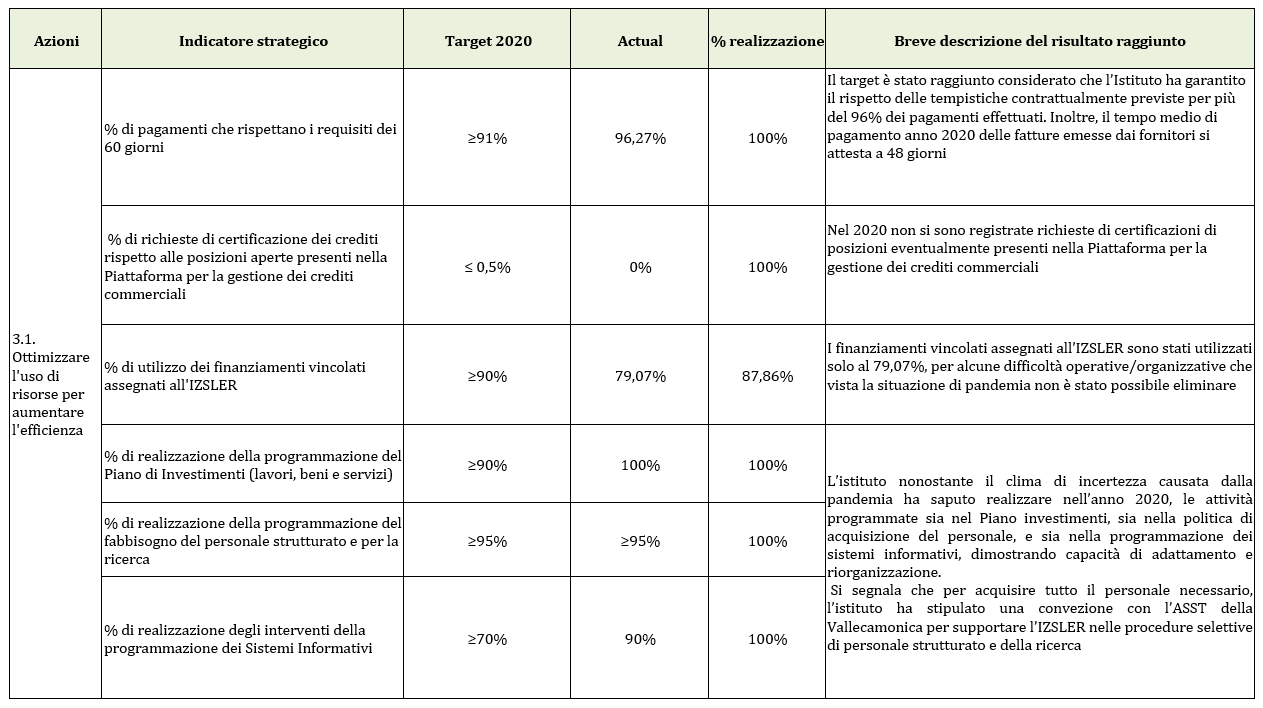
\includegraphics[width=1.1\linewidth]{figure/ob3} \end{center}

\newpage

\hypertarget{obiettivo-strategico-4-reingegnerizzazione-dei-processi}{%
\subsubsection*{\texorpdfstring{Obiettivo strategico 4:
\textbf{Reingegnerizzazione dei
processi}}{Obiettivo strategico 4: Reingegnerizzazione dei processi}}\label{obiettivo-strategico-4-reingegnerizzazione-dei-processi}}
\addcontentsline{toc}{subsubsection}{Obiettivo strategico 4:
\textbf{Reingegnerizzazione dei processi}}

Questo obiettivo è declinato in un'unica azione (obiettivo operativo):

-1 Sviluppare il processo di pianificazione, programmazione e controllo
con l'ottimizzazione dei processi trasversali tecnico scientifico ed
amministrativi

\begin{center}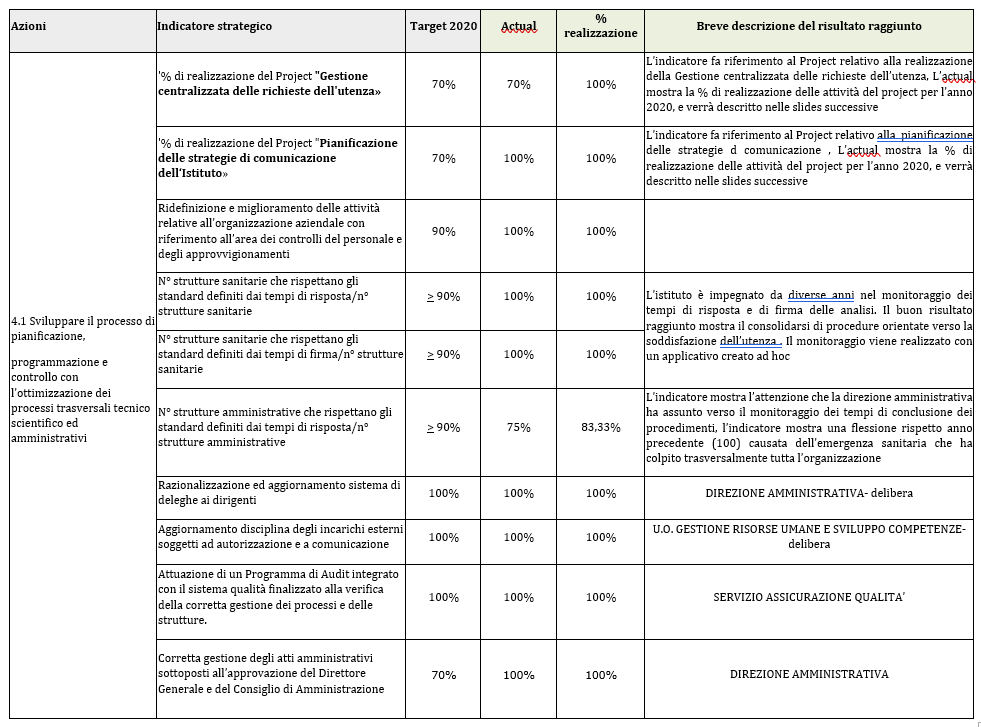
\includegraphics[width=1.1\linewidth]{figure/ob4} \end{center}

\newpage

\hypertarget{obiettivo-strategico-5-amministrazione-trasparente-ed-anticorruzione}{%
\subsubsection*{\texorpdfstring{Obiettivo strategico 5:
\textbf{Amministrazione trasparente ed
anticorruzione}}{Obiettivo strategico 5: Amministrazione trasparente ed anticorruzione}}\label{obiettivo-strategico-5-amministrazione-trasparente-ed-anticorruzione}}
\addcontentsline{toc}{subsubsection}{Obiettivo strategico 5:
\textbf{Amministrazione trasparente ed anticorruzione}}

Questo obiettivo è declinato in un'unica azione (obiettivo operativo) e
un solo indicatore:

-1 Adozione misure previste dalla normativa in materia di trasparenza e
prevenzione della corruzione

\begin{center}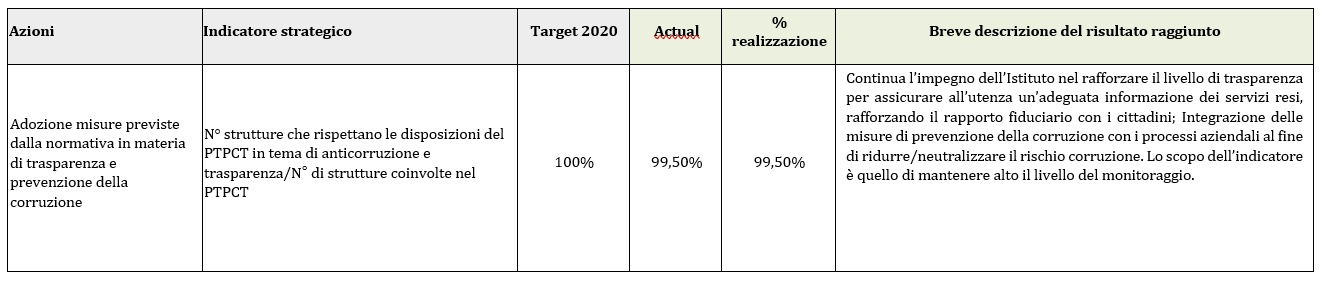
\includegraphics[width=1.1\linewidth]{figure/ob5} \end{center}

\newpage

\hypertarget{obiettivo-strategico-6-valorizzazione-del-capitale-umano}{%
\subsubsection*{\texorpdfstring{Obiettivo strategico 6:
\textbf{Valorizzazione del capitale
umano}}{Obiettivo strategico 6: Valorizzazione del capitale umano}}\label{obiettivo-strategico-6-valorizzazione-del-capitale-umano}}
\addcontentsline{toc}{subsubsection}{Obiettivo strategico 6:
\textbf{Valorizzazione del capitale umano}}

Questo obiettivo è declinato in due azioni (obiettivi operativi):

-1 Qualificazione e formazione del capitale umano;

-2 Efficacia ed efficienza degli interventi per la valorizzazione del
capitale umano

\begin{center}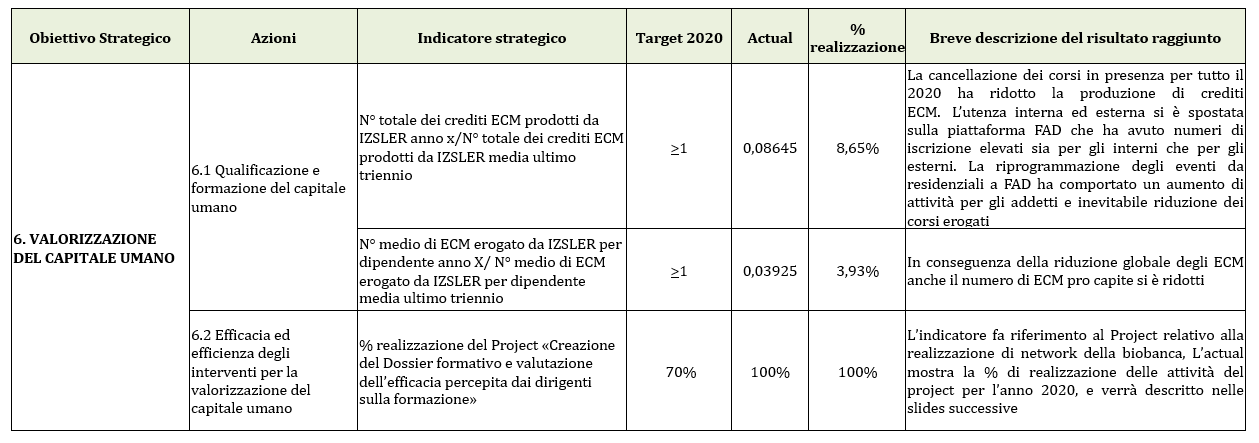
\includegraphics[width=1.1\linewidth]{figure/ob6} \end{center}

\textbf{E' necessario precisare che l'intero processo del ciclo di
gestione delle performance ha subito non poche difficoltà a causa
dell'emergenza sanitaria da COVID-19, che ha comportato un ritardo delle
sue fasi e un impatto sul raggiungimento di alcuni obiettivi. Nel corso
dell'anno 2020 l'Istituto è stato impegnato principalmente nel
fronteggiare la pandemia, destinando risorse, capacità e competenze a
tal fine, ritardando progetti e sospendendo altre attività.}

\hypertarget{il-cascading-dagli-obiettivi-strategici-agli-obiettivi-operativi}{%
\subsection{Il Cascading: dagli obiettivi strategici agli obiettivi
operativi}\label{il-cascading-dagli-obiettivi-strategici-agli-obiettivi-operativi}}

Dagli obiettivi strategici sono stati «costruiti» gli obiettivi
operativi inseriti all'interno dell' Albero della Performance in un
processo definito di «cascading», declinati in indicatori, target e
strutture assegnatarie, suddivisi nella quattro principali prospettive
di analisi. Nella dimensione \textbf{Istituzioni, cittadini e
consumatori} l'Ente mette in evidenza il rafforzamento dell'IZSLER nel
settore della PA centrale, l'ampliamento delle attività nell'ambito
della collaborazione con le Regioni e gli Enti locali, il potenziamento
dell'integrazione con il Ministero e le Regioni, l' aumento del network
scientifico e della collaborazione scientifica sia a livello nazionale
ed internazionale, la partecipazione a progetti di ricerca, twinning e
il potenziamento dell'attività diagnostica e delle produzioni. Una
dimensione strategica dell'IZSLER che pone le basi per lo sviluppo di
scenari futuri, declinati in ben n.~95 indicatori di
mantenimento/potenziamento di attività. Nella dimensione
\textbf{economico-finanziario} l'IZSLER analizza la gestione
economica-finanziaria in un'ottica di contenimento delle uscite, di
razionalizzazione dell'utilizzo delle risorse, improntati al
perseguimento dell'efficienza, assicurando la massima efficacia. Nella
dimensione dei **processi interni*»\textbf{ l'Ente valuta il modo in cui
raggiungere un migliore efficienza dell'amministrazione, attraverso
l'adeguamento dei processi produttivi dei servizi alle ``migliori
pratiche'' (modelli di eccellenza e standard internazionali e
nazionali), mediante l'ottimizzazione della gestione, delle procedure e
dei processi, con particolare riferimento al contenimento ed alla
riduzione dei tempi di TDF/TDR , nonché all'ottimizzazione dei tempi dei
procedimenti amministrativi. Nella dimensione della }Innovazione ,
crescita e sviluppo organizzativo** rientrano gli indicatori relativi
alla qualità totale e soddisfazione delle aspettative dell'utenza, che
si declinano nella qualità e la quantità delle prestazioni e dei servizi
erogati, dello sviluppo qualitativo e quantitativo delle relazioni con i
cittadini, gli utenti , i destinatari dei servizi e la rilevazione del
grado di soddisfazione dei destinatari delle attività. Lo sviluppo
organizzativo viene supportato dalla costante innovazione dei sistemi
informativi e dalla valorizzazione del capitale umano mediante percorsi
di promozione delle competenze. Vista la necessaria integrazione tra gli
obiettivi del Piano della Performance e il PTPCT, in questa sezione
vengono riportati anche gli obiettivi in tema di trasparenza,
anticorruzione e conflitto di interessi. In questa sezione si realizza
l'effettiva pianificazione, il controllo delle performance e dei
processi, analizzati da diverse prospettive. Le quattro dimensioni
vengono valutati sia dal punto di vista del singolo indicatore rispetto
al suo trend storico, sia rispetto alla scala dei valori/dimensione a
cui appartengono , sia rispetto al grado di performance della singole
struttura . Utilizzando opportuni strumenti di indagine è possibile fare
un'analisi su molti livelli; i grafici qui di seguito riportati sono un
esempio della valutazione fatte periodicamente dall'IZSLER, anche al
fine di un continuo e costante monitoraggio.

\hypertarget{i-risultati-raggiunti}{%
\subsection{I risultati raggiunti}\label{i-risultati-raggiunti}}

Di seguito in tabella sono riportati i risultati raggiunti nel 2020 sia
per quello che riguarda gli Obiettivi Strategici sia per gli Obiettivi
Operativi.

\begin{center}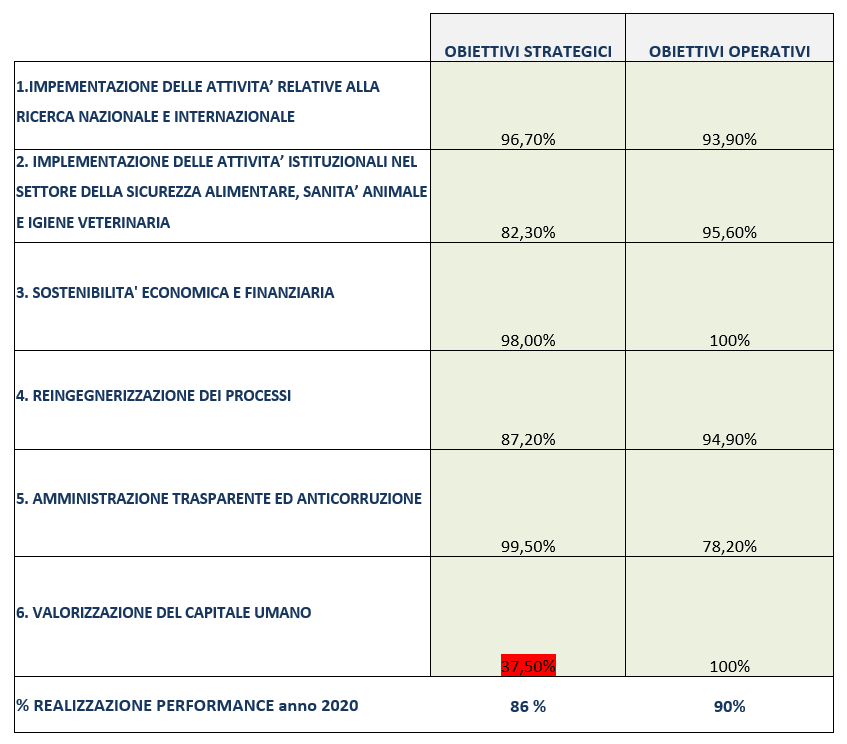
\includegraphics[width=0.9\linewidth]{figure/f8} \end{center}

\hypertarget{i-project}{%
\subsection{I project}\label{i-project}}

Cosa sono????

\textbf{PROJECT N.1: Realizzazione network nazionale ed internazionale
della Biobanca Veterinaria}

\emph{Significato strategico}:

\begin{itemize}
\tightlist
\item
  L'Istituto è sede di un biobanca veterinaria e centro di referenza OIE
  ''Veterinary Biobank'';
\item
  Il Ministero della Salute e l'OIE hanno ritenuto strategico realizzare
  a livello nazionale ed internazionale un network tra gli istituti di
  ricerca ed i centri di referenza nazionali ed internazionali;
\item
  L'Istituto ha avviato attività di pianificazione e programmazione per
  la realizzazione delle aspettative nazionali ed internazionali.
\end{itemize}

\emph{Sviluppo}:

\begin{itemize}
\tightlist
\item
  Azioni da realizzare a livello di Istituto e quindi di carattere
  trasversale alle strutture sanitarie ed amministrative;
\item
  Azioni di coordinamento nazionale con gli altri IIZZSS;
\item
  Azioni di pianificazione delle attività concordate con il Ministero e
  l'OIE.
\end{itemize}

\emph{Risultati attesi}:

\begin{itemize}
\tightlist
\item
  Realizzazione di un network nazionale;
\item
  Realizzazione della struttura informatica nazionale;
\item
  Integrazione del network nazionale con il progetto pilota
  internazionale;
\item
  Realizzazione della struttura informatica per la realizzazione del
  network internazionale
\item
  Disponibilità ai paesi terzi del modello di struttura informatica
  nazionale per l'integrazione con la piattaforma internazionale.
\end{itemize}

\emph{Attività realizzate nel 2020}:

\textbf{PROJECT N.2: Emissione e revisione metodi di prova}

\emph{Significato strategico}:

\begin{itemize}
\tightlist
\item
  L'Istituto persegue la politica della qualità da oltre vent'anni;
\item
  L'Unità Assicurazione Qualità è il supporto tecnico alle decisioni
  strategiche della direzione aziendale;
\item
  La decisione di avviare nuove attività, metodi di prova o variare il
  campo di applicazione degli stessi deve essere presa in coerenza con
  una strategia organizzativa.
\end{itemize}

\emph{Sviluppo}:

\begin{itemize}
\tightlist
\item
  Analisi dello stato attuale dell'accreditamento delle prove;
\item
  Analisi del grado di copertura dell'Istituto in relazione alle
  esigenze dei portatori di interesse istituzionali;
\item
  Definizione di una strategia operativa per il miglioramento del grado
  di copertura.
\end{itemize}

\emph{Risultati attesi}:\\
- Definizione di un sistema di verifica costante del grado di copertura
territoriale delle esigenze; - Ridistribuzione dei metodi analitici ed
eventuale revisione; - Programmazione delle modifiche dell'offerta
analitica dell'IZSLER

\emph{Attività realizzate nel 2020}:

\textbf{PROJECT N.3: Classyfarm}

\emph{Significato strategico}:

\begin{itemize}
\tightlist
\item
  Il Ministro della Salute ha identificato tra le linee prioritarie
  l'applicazione del sistema Classyfarm a livello nazionale;
\item
  L'IZSLER ha sviluppato per conto del Ministero della Salute il sistema
  classyfarm;
\item
  L'applicazione del sistema deve essere diffuso a livello nazionale ma
  deve avere la piena condivisione delle opportunità offerte anche
  all'interno di IZSLER.
\end{itemize}

\emph{Sviluppo}:

\begin{itemize}
\tightlist
\item
  Azioni da realizzare a livello di Istituto e quindi di carattere
  trasversale alle strutture sanitarie ed amministrative per
  l'applicazione del sistema;
\item
  Definizione delle azioni necessarie per consolidare il sistema
  all'Interno di IZSLER;
\item
  Azioni di coordinamento nazionale con gli altri IIZZSS;
\item
  Azioni di pianificazione delle attività concordate con il Ministero.
\end{itemize}

\emph{Risultati attesi}:

\begin{itemize}
\tightlist
\item
  Condivisione con tutte le strutture dell'IZSLER della strategicità
  delle azioni definite;
\item
  Creazione di percorsi operativi attraverso i quali sviluppare le
  attività dell'IZSLER;
\item
  Soddisfare le esigenze strategiche del Ministero per l'applicazione a
  livello nazionale.
\end{itemize}

\emph{Attività realizzate nel 2020}:

\textbf{PROJECT N.4: Gestione centralizzata delle richieste dell'utenza}
(integrato con il Project applicazione della lean alla gestione
centralizzata delle richieste dell'utenza)

\emph{Significato strategico}:

\begin{itemize}
\tightlist
\item
  L'Izsler ha definito nel piano di riorganizzazione una struttura
  strategica di gestione dell'interfaccia utente-IZSLER presso la sede
  centrale;
\item
  È opportuno razionalizzare l'utilizzo di risorse umane e strumentali
  dedicate;
\item
  È opportuno ridurre i punti di accettazioni presenti presso la sede di
  Brescia;
\item
  È opportuno separare le responsabilità accettazione e gestione
  conflitto di interessi.
\end{itemize}

\emph{Sviluppo}:

\begin{itemize}
\tightlist
\item
  Azioni da realizzare a livello di Istituto e quindi di carattere
  trasversale alle strutture sanitarie ed amministrative per la
  realizzazione della sede operativa unica;
\item
  Acquisizione di ulteriori fasi comuni utili alla razionalizzazione del
  processo di gestione e circolazione di campioni e dati;
\item
  Realizzazione di sistemi di monitoraggio e feedback verso i reparti di
  dati di gestione ed analisi dei tempi di realizzazione dei processi
  produttivi;
\item
  Semplificazione di procedure informatiche e di gestione del sistema
  qualità;
\item
  Collegamento operativo con le attività della biobanca.
\end{itemize}

\emph{Risultati attesi}:

\begin{itemize}
\tightlist
\item
  Realizzazione della sede unica per l'accettazione dei campioni,
  semplificazione nei rapporti con i clienti: front office unico e
  Uniformità di comportamenti;
\item
  Controllo quali-quantitativo flusso campioni e dati e alimentazione
  sistema informativo aziendale uniforme e coerente;
\item
  Realizzazione di un sistema di monitoraggio attività e tempi, feed
  back ai reparti e supporto per il miglioramento degli stessi;
\item
  Semplificazione dei processi e applicazione di sistemi di eliminazione
  delle attività non a valore per l'organizzazione.
\end{itemize}

\emph{Attività realizzate nel 2020}:

\textbf{PROJECT N.5: Pianificazione delle strategie di comunicazione
dell'Istituto}

\emph{Significato strategico}:

\begin{itemize}
\tightlist
\item
  L'Izsler ha definito nel piano di riorganizzazione un ufficio dedicato
  alla comunicazione;
\item
  Gli strumenti di comunicazione disponibili devono essere utilizzati in
  modo organizzato strutturato e secondo politiche predefinite;
\item
  La comunicazione verso l'esterno e verso l'esterno rappresenta un
  elemento determinante per valorizzare le attività svolte.
\end{itemize}

\emph{Sviluppo}:

\begin{itemize}
\tightlist
\item
  Realizzare azioni per pianificare e migliorare la comunicazione verso
  l'esterno;
\item
  Realizzare azioni per pianificare e migliorare la comunicazione verso
  l'interno;
\item
  Attivare un servizio interno di analisi e produzione delle
  informazioni.
\end{itemize}

\emph{Risultati attesi}:

\begin{itemize}
\tightlist
\item
  Revisione aggiornamento e pianificazione redazionale del sito
  istituzionale;
\item
  Attivazione della presenza sui social media;
\item
  Attivazione ed aggiornamento di una APP istituzionale;
\item
  Nuove modalità di interazione tra uffici e reparti.
\end{itemize}

\emph{Attività realizzate nel 2020}:

\hypertarget{gli-obiettivi-individuali-direzione-generale-sanitaria-ed-amministrativa}{%
\section{Gli Obiettivi Individuali: Direzione Generale, Sanitaria ed
Amministrativa}\label{gli-obiettivi-individuali-direzione-generale-sanitaria-ed-amministrativa}}

La Giunta della Regione Lombardia con deliberazione n.~XI/2110 del
09.09.2019, ha definito, di concerto con la Regione Emilia Romagna, gli
obiettivi aziendali di interesse regionale per l'anno di riferimento del
Direttore Generale dell'Istituto. Con Decreto n.~305 del 24.09.2019 il
Direttore Generale, prende atto del coinvolgimento del Direttore
Amministrativo e del Direttore Sanitario nel raggiungimento degli
obiettivi per l'anno 2020.Al Direttore Sanitario e al Direttore
Amministrativo, oltre agli obiettivi aziendali di interesse regionali,
sono stati assegnati anche gli obiettivi strategici che per i diversi
ambiti di competenza li riguardavano. Con nota prot. N. 1967 del
31/01/2020 è stata trasmessa alle Regione la rendicontazione attestante
l'attività svolta per ciascun obiettivo. Al momento non è ancora stato
comunicato dalle Regioni la valutazione sul raggiungimento degli
obiettivi assegnati per l'anno 2020

\hypertarget{gli-elementi-di-valutazione-quantitativa-e-qualitativa}{%
\subsection{Gli elementi di valutazione quantitativa e
qualitativa}\label{gli-elementi-di-valutazione-quantitativa-e-qualitativa}}

Le schede di valutazione individuale sono state redatte in conformità
alle metodologie indicate nel Sistema di Misurazione e Valutazione
dell'IZSLER anno 2020, approvato con delibera del direttore generale
n.\_\_ del\_\_\_. In base alla normativa vigente e agli accordi
aziendali, i responsabili di struttura hanno regolarmente provveduto
alla valutazione del personale dirigente e di comparto. Si presenta qui
di seguito gli elementi costitutivi della schede di valutazione del
personale del comparto e della dirigenza.

\begin{center}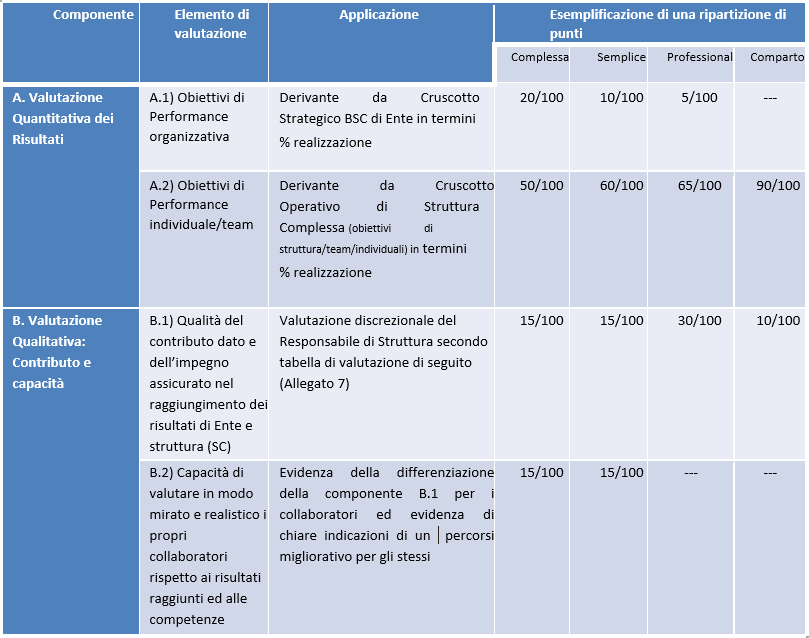
\includegraphics[width=0.9\linewidth]{figure/f3} \end{center}

\hypertarget{elementi-di-valutazione-qualitativa-le-aree-di-attenzione}{%
\subsubsection{Elementi di valutazione qualitativa: le aree di
attenzione}\label{elementi-di-valutazione-qualitativa-le-aree-di-attenzione}}

\textbf{Valutazione Qualitativa}: relativa alla qualità del contributo
dato e dell'impegno assicurato al raggiungimento degli obiettivi
assegnati. I criteri di valutazione sono differenziati tra personale del
Comparto e della Dirigenza, ed all'interno di quest'ultima tra Dirigenti
Responsabili di Struttura e Professional, come di seguito illustrato.
\textbf{Personale del Comparto}: La valutazione qualitativa del
contributo dato e dell'impegno assicurato nell'anno di riferimento è
valutata con riferimento alle aree di attenzione previste per la
categoria di appartenenza e specificate nella scheda di assegnazione
come sotto riportate. Il Valutatore descrive brevemente il contributo
atteso in relazione ad ognuna delle aree identificate ed agli obiettivi
assegnati e il giudizio finale deve essere oggettivabile anche
documentalmente.

\begin{center}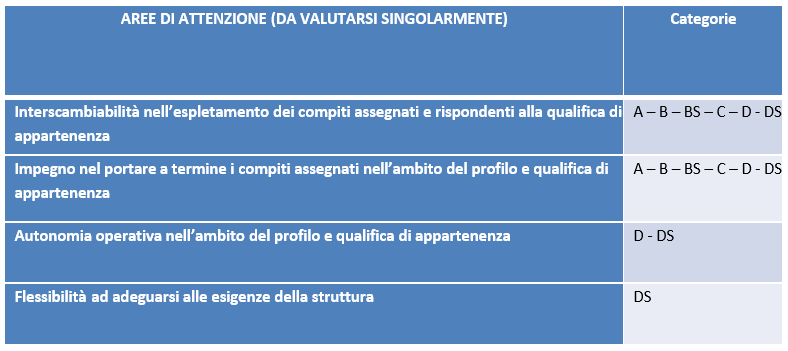
\includegraphics[width=0.9\linewidth]{figure/f4} \end{center}

\textbf{Dirigenti delle aree Veterinaria - Sanitaria - Tecnica -
Professionale - Amministrativa.} Sono state individuate n.~9 aree di
attenzione, tra le quali il Valutatore può scegliere per il Dirigente
valutato non meno di 3 e non più di 5 aree tra le n.~9 elencate. Anche
in questo caso il Valutatore descrive brevemente il contributo atteso in
relazione ad ognuna delle aree identificate ed agli obiettivi assegnati
e il giudizio finale complessivo per tutte le aree individuate deve
essere oggettivabile anche documentalmente.

\begin{center}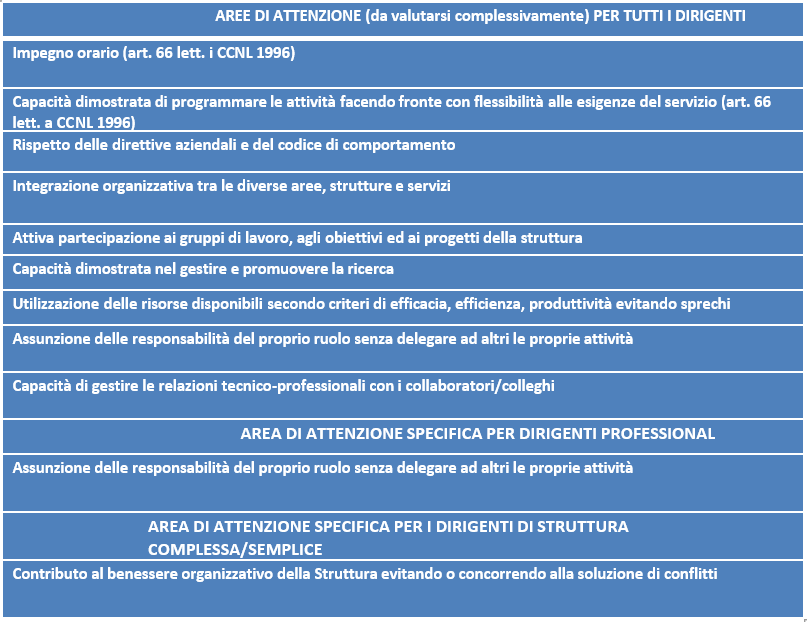
\includegraphics[width=0.9\linewidth]{figure/f5} \end{center}

\hypertarget{azioni-svolte-nellambito-del-ptpct}{%
\section{Azioni svolte nell'ambito del
PTPCT}\label{azioni-svolte-nellambito-del-ptpct}}

Il quadro normativo sulla prevenzione della corruzione e sulla
trasparenza ha sempre evidenziato l'importanza di integrare il ciclo
della Performance con gli strumenti ed i processi relativi alla qualità
dei servizi, alla trasparenza, all'integrità e in generale alla
prevenzione della corruzione. Per rendere efficace tale collegamento nel
PTPCT è stato inserito un cronoprogramma di obiettivi da perseguire nel
Piano Performance 2020-2022. Tali obiettivi sono stati assegnati alle
varie strutture. Si riporta qui di seguito il cronoprogramma:

INSERIRE IL CRONOPROGRAMMA

Inoltre, In applicazione della L. n.~190/2012 in materia di prevenzione
della corruzione e del D. L.gs n.~33/2013 di riordino degli obblighi di
pubblicità, trasparenza e diffusioni di informazioni da parte delle
Pubbliche Amministrazioni, l'IZSLER ha adottato i seguenti
provvedimenti:

\begin{itemize}
\tightlist
\item
  con deliberazione n.~7 del 5.7.2016 il Consiglio di Amministrazione ha
  nominato la dott.ssa Lauretta Cocchi, Responsabile della Prevenzione
  della Corruzione e della Trasparenza;
\item
  con delibera del Consiglio di Amministrazione n.~13 del 30.10.2017 ha
  recepito il Codice di Comportamento dei dipendenti dell'IZSLER;
\item
  con delibera del Consiglio di Amministrazione n.~1 del 29.01.2018 ha
  approvato il Piano Triennale di Prevenzione della Corruzione e della
  Trasparenza 2018 -- 2020; La sezione Amministrazione Trasparente del
  sito istituzionale è stata regolarmente aggiornata. In particolare si
  segnala la pubblicazione dei seguenti documenti:
\item
  in data 31.0.1.2019: Relazione annuale al 31/12/2018 del Responsabile
  della Prevenzione della Corruzione - Art. Comma 14, Legge
  6.11.2012/190; in data 10.04.2018: Attestazione del Nucleo di
  Valutazione delle Prestazioni dell'Istituto sull'assolvimento degli
  obblighi di pubblicazione ex Delibera ANAC 141/2018 al 31/03/2018.
  Integrazione del sistema anticorruzione con il sistema qualità
\end{itemize}

\hypertarget{il-processo-di-redazione-della-relazione-sulla-performance}{%
\section{Il processo di redazione della relazione sulla
performance}\label{il-processo-di-redazione-della-relazione-sulla-performance}}

\begin{center}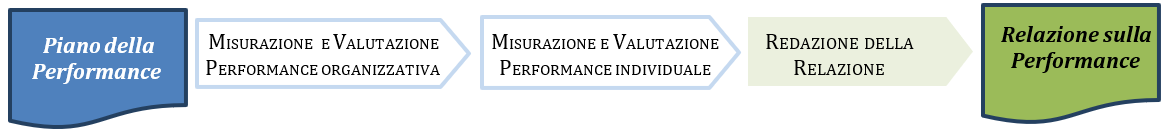
\includegraphics[width=0.9\linewidth]{figure/f7} \end{center}

Il supporto al funzionamento del ciclo di gestione delle performance è
assicurato dall'U.O. Gestione del Personale, il quale assicura inoltre
le attività connesse al Sistema di Valutazione del Personale. Il
supporto informatico è assicurato dai Sistemi Informativi che
cominciando dal 2013 hanno implementato la prima sperimentazione del
cruscotto per la gestione del ciclo delle performance. Dal 2014 in
sinergia tra l'U.O. Gestione del Personale e Sistemi Informativi si è
sviluppato una nuova tipologia di cruscotto denominato «Obiettivi
Strategici» e sono state predisposte le basi dati di appoggio per il
caricamento dei target da parte delle strutture assegnatarie degli
obiettivi/indicatori.Lo stesso è stato accompagnato da un altro
applicativo che ha consentito, anche se in modo sperimentale, di
implementare lo stato d'avanzamento delle attività e le percentuali di
conseguimento dei target rispetto a quelli prefissati, dandone anche un
evidenza grafica.

\hypertarget{conclusioni}{%
\section{Conclusioni}\label{conclusioni}}

La Relazione sulla Performance è un documento di sintesi dell'intero
ciclo di gestione della performance riferito ad un ciclo amministrativo.
E' anche un'opportunità per analizzare la validità e l'efficacia del
processo e per fornire possibili input di miglioramento.

Il 2020 è stato un anno di difficile attuazione per la situazione
pandemica mondiale che ha visto l'Istituto impegnato in prima linea
nell'affrontare tale emergenza, comportando un ritardo nella
negoziazione, nell'assegnazione degli obiettivi e negli steps
successivi.

E' da evidenziare lo sforzo compiuto da tutto il personale fin
dall'inizio dell'emergenza, che ha saputo riadattare le proprie attività
lavorative, anche con la sperimentazione di nuove modalità di lavoro
``smart working'' con risultati positivi, reagendo con prontezza e
disponibilità al periodo difficile che abbiamo vissuto.

\begin{verbatim}
                                            IL DIRETTORE GENERALE
                                                  Dr. Piero Frazzi
\end{verbatim}

\end{document}
